% Options for packages loaded elsewhere
\PassOptionsToPackage{unicode}{hyperref}
\PassOptionsToPackage{hyphens}{url}
%
\documentclass[
]{article}
\usepackage{amsmath,amssymb}
\usepackage{lmodern}
\usepackage{iftex}
\ifPDFTeX
  \usepackage[T1]{fontenc}
  \usepackage[utf8]{inputenc}
  \usepackage{textcomp} % provide euro and other symbols
\else % if luatex or xetex
  \usepackage{unicode-math}
  \defaultfontfeatures{Scale=MatchLowercase}
  \defaultfontfeatures[\rmfamily]{Ligatures=TeX,Scale=1}
\fi
% Use upquote if available, for straight quotes in verbatim environments
\IfFileExists{upquote.sty}{\usepackage{upquote}}{}
\IfFileExists{microtype.sty}{% use microtype if available
  \usepackage[]{microtype}
  \UseMicrotypeSet[protrusion]{basicmath} % disable protrusion for tt fonts
}{}
\makeatletter
\@ifundefined{KOMAClassName}{% if non-KOMA class
  \IfFileExists{parskip.sty}{%
    \usepackage{parskip}
  }{% else
    \setlength{\parindent}{0pt}
    \setlength{\parskip}{6pt plus 2pt minus 1pt}}
}{% if KOMA class
  \KOMAoptions{parskip=half}}
\makeatother
\usepackage{xcolor}
\IfFileExists{xurl.sty}{\usepackage{xurl}}{} % add URL line breaks if available
\IfFileExists{bookmark.sty}{\usepackage{bookmark}}{\usepackage{hyperref}}
\hypersetup{
  pdftitle={Google Data Analytics Capstone Project - Cyclistic},
  pdfauthor={Samsil Arifeen},
  hidelinks,
  pdfcreator={LaTeX via pandoc}}
\urlstyle{same} % disable monospaced font for URLs
\usepackage[margin=1in]{geometry}
\usepackage{color}
\usepackage{fancyvrb}
\newcommand{\VerbBar}{|}
\newcommand{\VERB}{\Verb[commandchars=\\\{\}]}
\DefineVerbatimEnvironment{Highlighting}{Verbatim}{commandchars=\\\{\}}
% Add ',fontsize=\small' for more characters per line
\usepackage{framed}
\definecolor{shadecolor}{RGB}{248,248,248}
\newenvironment{Shaded}{\begin{snugshade}}{\end{snugshade}}
\newcommand{\AlertTok}[1]{\textcolor[rgb]{0.94,0.16,0.16}{#1}}
\newcommand{\AnnotationTok}[1]{\textcolor[rgb]{0.56,0.35,0.01}{\textbf{\textit{#1}}}}
\newcommand{\AttributeTok}[1]{\textcolor[rgb]{0.77,0.63,0.00}{#1}}
\newcommand{\BaseNTok}[1]{\textcolor[rgb]{0.00,0.00,0.81}{#1}}
\newcommand{\BuiltInTok}[1]{#1}
\newcommand{\CharTok}[1]{\textcolor[rgb]{0.31,0.60,0.02}{#1}}
\newcommand{\CommentTok}[1]{\textcolor[rgb]{0.56,0.35,0.01}{\textit{#1}}}
\newcommand{\CommentVarTok}[1]{\textcolor[rgb]{0.56,0.35,0.01}{\textbf{\textit{#1}}}}
\newcommand{\ConstantTok}[1]{\textcolor[rgb]{0.00,0.00,0.00}{#1}}
\newcommand{\ControlFlowTok}[1]{\textcolor[rgb]{0.13,0.29,0.53}{\textbf{#1}}}
\newcommand{\DataTypeTok}[1]{\textcolor[rgb]{0.13,0.29,0.53}{#1}}
\newcommand{\DecValTok}[1]{\textcolor[rgb]{0.00,0.00,0.81}{#1}}
\newcommand{\DocumentationTok}[1]{\textcolor[rgb]{0.56,0.35,0.01}{\textbf{\textit{#1}}}}
\newcommand{\ErrorTok}[1]{\textcolor[rgb]{0.64,0.00,0.00}{\textbf{#1}}}
\newcommand{\ExtensionTok}[1]{#1}
\newcommand{\FloatTok}[1]{\textcolor[rgb]{0.00,0.00,0.81}{#1}}
\newcommand{\FunctionTok}[1]{\textcolor[rgb]{0.00,0.00,0.00}{#1}}
\newcommand{\ImportTok}[1]{#1}
\newcommand{\InformationTok}[1]{\textcolor[rgb]{0.56,0.35,0.01}{\textbf{\textit{#1}}}}
\newcommand{\KeywordTok}[1]{\textcolor[rgb]{0.13,0.29,0.53}{\textbf{#1}}}
\newcommand{\NormalTok}[1]{#1}
\newcommand{\OperatorTok}[1]{\textcolor[rgb]{0.81,0.36,0.00}{\textbf{#1}}}
\newcommand{\OtherTok}[1]{\textcolor[rgb]{0.56,0.35,0.01}{#1}}
\newcommand{\PreprocessorTok}[1]{\textcolor[rgb]{0.56,0.35,0.01}{\textit{#1}}}
\newcommand{\RegionMarkerTok}[1]{#1}
\newcommand{\SpecialCharTok}[1]{\textcolor[rgb]{0.00,0.00,0.00}{#1}}
\newcommand{\SpecialStringTok}[1]{\textcolor[rgb]{0.31,0.60,0.02}{#1}}
\newcommand{\StringTok}[1]{\textcolor[rgb]{0.31,0.60,0.02}{#1}}
\newcommand{\VariableTok}[1]{\textcolor[rgb]{0.00,0.00,0.00}{#1}}
\newcommand{\VerbatimStringTok}[1]{\textcolor[rgb]{0.31,0.60,0.02}{#1}}
\newcommand{\WarningTok}[1]{\textcolor[rgb]{0.56,0.35,0.01}{\textbf{\textit{#1}}}}
\usepackage{graphicx}
\makeatletter
\def\maxwidth{\ifdim\Gin@nat@width>\linewidth\linewidth\else\Gin@nat@width\fi}
\def\maxheight{\ifdim\Gin@nat@height>\textheight\textheight\else\Gin@nat@height\fi}
\makeatother
% Scale images if necessary, so that they will not overflow the page
% margins by default, and it is still possible to overwrite the defaults
% using explicit options in \includegraphics[width, height, ...]{}
\setkeys{Gin}{width=\maxwidth,height=\maxheight,keepaspectratio}
% Set default figure placement to htbp
\makeatletter
\def\fps@figure{htbp}
\makeatother
\setlength{\emergencystretch}{3em} % prevent overfull lines
\providecommand{\tightlist}{%
  \setlength{\itemsep}{0pt}\setlength{\parskip}{0pt}}
\setcounter{secnumdepth}{-\maxdimen} % remove section numbering
\ifLuaTeX
  \usepackage{selnolig}  % disable illegal ligatures
\fi

\title{Google Data Analytics Capstone Project - Cyclistic}
\author{Samsil Arifeen}
\date{2022-03-13}

\begin{document}
\maketitle

\hypertarget{introduction}{%
\section{\texorpdfstring{\textbf{Introduction}}{Introduction}}\label{introduction}}

This is a case study that i conducted to solve for Google data analytics
certifications Course Capstone Project: Case Study 1 ``Cyclistic''. This
is my first ever case study on data analytics as well. It involves a
fictional bike share company based in Chicago, USA. However the company
wants to know the different users' behavior while using the services
available. The management believes that doing this, they will be able to
start a new marketing strategy that will be key for future growth of the
company. As I have learned from the Google Data Analytics program, I
will follow the steps of the data analysis process: ask, prepare,
process, analyze, share and act. However, since act step is for
executives to decide, I will not cover that step in this solution.

\hypertarget{scenario}{%
\section{\texorpdfstring{\textbf{Scenario}}{Scenario}}\label{scenario}}

Cyclistic operates a fleet of more than 5,800 bicycles which can be
accessed from over 600 docking stations across the city. Bikes can be
borrowed from one docking station, ridden, then returned to any docking
stations. Over the years marketing campaigns have been broad and
targeted a cross-section of potential users. Data analysis has shown
that riders with an annual membership are more profitable than casual
riders. Lily Moreno, the director of marketing, wants to implement a new
marketing strategy in order to convert casual riders into annual
members. She believes that with the right campaign there is a very good
chance of such conversions between the user types. There are also
user-friendly bike options include such as electric bikes, classic bikes
and docked bikes. It makes Cyclistic services more inclusive to people.
Lily has tasked the marketing analytics team to analyze past user data
of one year to find trends and habits of Cyclistic's users to help
create this marketing campaign. The marketing analyst team would like to
know:

\begin{itemize}
\tightlist
\item
  how annual members and casual riders differ
\item
  why casual riders would buy a membership
\item
  how Cyclistic can use digital media to influence casual riders to
  become members.
\end{itemize}

Here i have to analyze the Cyclistic historical bike trip data to
identify trends in the usage of bikes by casual and member riders.

\hypertarget{phase-1-ask}{%
\section{\texorpdfstring{\textbf{Phase 1:
Ask}}{Phase 1: Ask}}\label{phase-1-ask}}

\hypertarget{business-objective}{%
\paragraph{\texorpdfstring{\textbf{Business
objective}}{Business objective}}\label{business-objective}}

To increase profitability by converting casual riders to annual members
via a targeted marketing campaign.

\hypertarget{business-task}{%
\paragraph{\texorpdfstring{\textbf{Business
task}}{Business task}}\label{business-task}}

The junior analyst has been tasked with answering this question:

\begin{itemize}
\tightlist
\item
  How do \textbf{annual members} and \textbf{casual riders} use
  Cyclistic bikes differently? The behavioral differences between annual
  members and casual riders.
\item
  Why a \textbf{casual rider} would buy Cyclistic \textbf{annual
  memberships}.
\item
  How digital media can influence \textbf{casual riders} to becoming
  \textbf{annual members}.
\end{itemize}

The marketing analytics team tasked me with using past user data to find
the behavioral differences between annual members and casual riders and
report their findings.

\hypertarget{stakeholders}{%
\paragraph{\texorpdfstring{\textbf{Stakeholders}}{Stakeholders}}\label{stakeholders}}

The stakeholders in this project include:

\begin{itemize}
\item
  Lily Moreno, Director of Marketing at Cyclistic, who is responsible
  for implementing the marketing campaigns at Cyclistic.
\item
  The Cyclistic marketing analytics team. This team is responsible for
  collecting, analyzing and reporting data to be used in marketing
  campaigns. I am the junior analyst in this team.
\item
  The Cyclistic executive team. This team makes the final decision on
  the recommended marketing plan. They are notoriously detail-oriented.
\end{itemize}

\hypertarget{phase-2-prepare}{%
\section{\texorpdfstring{\textbf{Phase 2:
Prepare}}{Phase 2: Prepare}}\label{phase-2-prepare}}

\hypertarget{where-is-data-located}{%
\paragraph{\texorpdfstring{\textbf{Where is Data
located}}{Where is Data located}}\label{where-is-data-located}}

The data used for this analysis were obtained from the Motivate, a
company employed by the City of Chicago to collect data on bike share
usage. Here is the
\href{https://divvy-tripdata.s3.amazonaws.com/index.html}{link} for the
datasets that i have used in this case study.

\hypertarget{how-is-the-data-organized}{%
\paragraph{\texorpdfstring{\textbf{How is the Data
Organized?}}{How is the Data Organized?}}\label{how-is-the-data-organized}}

The data is organized in monthly csv files. The most recent twelve
months of data (December, 2020 -- November,2021) were used for this
project. The files consist of 13 columns containing information related
to ride id, ridership type, ride time, start location and end location
and geographic coordinates, etc.

\hypertarget{credibility-of-the-data}{%
\paragraph{\texorpdfstring{\textbf{Credibility of the
Data}}{Credibility of the Data}}\label{credibility-of-the-data}}

The \href{https://divvy-tripdata.s3.amazonaws.com/index.html}{data} is
collected directly by Motivate, Inc., the company that runs the
Cyclistic Bike Share program for the City of Chicago. The data is
comprehensive and consistent as it consists of data for all the rides
taken by users and it is not just a sample of the data. The data is
current as it had been released monthly. The City of Chicago makes the
data available to the public.

\hypertarget{licensing-privacy-security-and-accessibility}{%
\paragraph{\texorpdfstring{\textbf{Licensing, privacy, security, and
accessibility}}{Licensing, privacy, security, and accessibility}}\label{licensing-privacy-security-and-accessibility}}

This \href{https://divvy-tripdata.s3.amazonaws.com/index.html}{data} has
been stripped of all identifying information. This ensures privacy, but
it limits the extent of the possible analysis. There is not enough data
to determine if casual riders are repeat-riders or if casual riders are
residents of the Chicago area. The data is released under this
\href{https://ride.divvybikes.com/data-license-agreement}{license}.

\hypertarget{ability-of-data-to-answer-business-questions}{%
\paragraph{\texorpdfstring{\textbf{Ability of Data to answer Business
Questions}}{Ability of Data to answer Business Questions}}\label{ability-of-data-to-answer-business-questions}}

In order to answer the business question, How do \textbf{annual members}
and \textbf{casual riders} use Cyclistic bikes differently,The
behavioral differences between annual members and casual riders, the
available dataset is sufficient enough. After a detail observation about
the variables, it is clearly depicted that casual riders pay for
individual or daily rides whereas members riders purchase annual
subscriptions. This information is very important in order to determine
the behavioral differences between the two groups.

\hypertarget{challenges-with-the-data}{%
\paragraph{\texorpdfstring{\textbf{Challenges with the
data}}{Challenges with the data}}\label{challenges-with-the-data}}

\begin{itemize}
\item
  There are some problems with the data as well. Most of the the
  problems (duplicate records, missing fields, etc.) can be dealt with
  by data cleaning.
\item
  There was 12 csv files for 12 months/year. After combining all the
  files, it became 1.2 Gb in total size. It was alright until it became
  larger than my laptop's RAM. At first i tried to dealt it with
  diskframe function, but as it took too long for me to learn and apply
  i have decided to go by segments. In that case, i did the data
  cleaning and then removed all the variables that i am not going to
  work with at this moment. Then i wrote it down in a csv file in the
  hard disk and imported it again for analysis and preparing
  visualization.
\end{itemize}

\hypertarget{phase-3-data-process}{%
\section{\texorpdfstring{\textbf{Phase 3: Data
Process}}{Phase 3: Data Process}}\label{phase-3-data-process}}

\hypertarget{what-tools-are-you-choosing-and-why}{%
\paragraph{\texorpdfstring{\textbf{What tools are you choosing and
why?}}{What tools are you choosing and why?}}\label{what-tools-are-you-choosing-and-why}}

For this project I choose RStudio Desktop in order to prepare, process,
clean, analyze and create the visualizations. The data set was too large
to be processed in Ms Excel, google spreadsheets and RStudio Cloud.

\hypertarget{review-of-data}{%
\paragraph{\texorpdfstring{\textbf{Review of
Data}}{Review of Data}}\label{review-of-data}}

In order to get an overview, the data was reviewed in terms of
understanding of the concent of variables, data formats and data
integrity.

Data review involved the following:

\begin{itemize}
\tightlist
\item
  Checking column names across all the 12 original files.
\item
  Checking for missing values.
\item
  Checking of white spaces.
\item
  Checking of duplicate records.
\item
  Other data anomalies.
\end{itemize}

However the review of the data revealed several problems:

\begin{itemize}
\tightlist
\item
  Duplicate record of ID numbers.
\item
  Records with missing start or end station name.
\item
  Records with very short or very long ride duration.
\item
  Records for trips starting or ending at an administrative station
  (repair or testing station)
\end{itemize}

All 12 files were combined into one data set after initial review was
completed.The final data set consisted of 5479096 rows with 13 columns
of character and numeric data. This matched the number of records in all
12 monthly data files.

\hypertarget{setting-up-environment}{%
\paragraph{\texorpdfstring{\textbf{Setting up
environment}}{Setting up environment}}\label{setting-up-environment}}

\begin{Shaded}
\begin{Highlighting}[]
\CommentTok{\# Setting working directory}
\FunctionTok{setwd}\NormalTok{(}\StringTok{"/home/samsil/Documents/CaseStudy1{-}Cyclistic/"}\NormalTok{)}

\CommentTok{\#install packages}
\FunctionTok{install.packages}\NormalTok{(}\StringTok{\textquotesingle{}tidyverse\textquotesingle{}}\NormalTok{)}
\FunctionTok{install.packages}\NormalTok{(}\StringTok{"janitor"}\NormalTok{) }
\FunctionTok{install.packages}\NormalTok{(}\StringTok{"lubridate"}\NormalTok{)}
\FunctionTok{install.packages}\NormalTok{(}\StringTok{"devtools"}\NormalTok{)}
\FunctionTok{install.packages}\NormalTok{(}\StringTok{"psych"}\NormalTok{)}

\CommentTok{\#load packages}

\FunctionTok{library}\NormalTok{(tidyverse)}
\FunctionTok{library}\NormalTok{(lubridate)}
\FunctionTok{library}\NormalTok{(janitor)}
\FunctionTok{library}\NormalTok{(data.table)}
\FunctionTok{library}\NormalTok{(readr)}
\FunctionTok{library}\NormalTok{(psych)}
\CommentTok{\#{-}{-}{-}{-}{-}{-}{-}{-}{-}{-}{-}{-}{-}{-}{-}{-}{-}{-}{-}{-}{-}{-}{-}{-}{-}{-}{-}{-}{-}{-}{-}{-}{-}{-}{-}{-}{-}{-}{-}{-}{-}{-}{-}{-}{-}{-}{-}{-}{-}{-}{-}{-}{-}{-}{-}{-}{-}{-}{-}{-}{-}{-}{-}{-}{-}{-}{-}{-}{-}{-}{-}}
\end{Highlighting}
\end{Shaded}

\hypertarget{collect-datadata-wrangling}{%
\paragraph{\texorpdfstring{\textbf{Collect Data(Data
wrangling)}}{Collect Data(Data wrangling)}}\label{collect-datadata-wrangling}}

\begin{itemize}
\tightlist
\item
  At this point, i had to upload data files into new vectors and we will
  run it only once to combine out data frames into one big dataset.
\end{itemize}

\begin{Shaded}
\begin{Highlighting}[]
\NormalTok{december\_2020 }\OtherTok{\textless{}{-}} \FunctionTok{read.csv}\NormalTok{(}\StringTok{"202012{-}divvy{-}tripdata.csv"}\NormalTok{)}
\NormalTok{january\_2021 }\OtherTok{\textless{}{-}} \FunctionTok{read.csv}\NormalTok{(}\StringTok{"202101{-}divvy{-}tripdata.csv"}\NormalTok{)}
\NormalTok{february\_2021 }\OtherTok{\textless{}{-}} \FunctionTok{read.csv}\NormalTok{(}\StringTok{"202102{-}divvy{-}tripdata.csv"}\NormalTok{)}
\NormalTok{march\_2021 }\OtherTok{\textless{}{-}} \FunctionTok{read.csv}\NormalTok{(}\StringTok{"202103{-}divvy{-}tripdata.csv"}\NormalTok{)}
\NormalTok{april\_2021 }\OtherTok{\textless{}{-}} \FunctionTok{read.csv}\NormalTok{(}\StringTok{"202104{-}divvy{-}tripdata.csv"}\NormalTok{)}
\NormalTok{may\_2021 }\OtherTok{\textless{}{-}} \FunctionTok{read.csv}\NormalTok{(}\StringTok{"202105{-}divvy{-}tripdata.csv"}\NormalTok{) }
\NormalTok{june\_2021 }\OtherTok{\textless{}{-}} \FunctionTok{read.csv}\NormalTok{(}\StringTok{"202106{-}divvy{-}tripdata.csv"}\NormalTok{)}
\NormalTok{july\_2021 }\OtherTok{\textless{}{-}} \FunctionTok{read.csv}\NormalTok{(}\StringTok{"202107{-}divvy{-}tripdata.csv"}\NormalTok{)}
\NormalTok{august\_2021 }\OtherTok{\textless{}{-}} \FunctionTok{read.csv}\NormalTok{(}\StringTok{"202108{-}divvy{-}tripdata.csv"}\NormalTok{)}
\NormalTok{september\_2021 }\OtherTok{\textless{}{-}} \FunctionTok{read.csv}\NormalTok{(}\StringTok{"202109{-}divvy{-}tripdata.csv"}\NormalTok{)}
\NormalTok{october\_2021 }\OtherTok{\textless{}{-}} \FunctionTok{read.csv}\NormalTok{(}\StringTok{"202110{-}divvy{-}tripdata.csv"}\NormalTok{)}
\NormalTok{november\_2021 }\OtherTok{\textless{}{-}} \FunctionTok{read.csv}\NormalTok{(}\StringTok{"202111{-}divvy{-}tripdata.csv"}\NormalTok{)}
\CommentTok{\#{-}{-}{-}{-}{-}{-}{-}{-}{-}{-}{-}{-}{-}{-}{-}{-}{-}{-}{-}{-}{-}{-}{-}{-}{-}{-}{-}{-}{-}{-}{-}{-}{-}{-}{-}{-}{-}{-}{-}{-}{-}{-}{-}{-}{-}{-}{-}{-}{-}{-}{-}{-}{-}{-}{-}{-}{-}{-}{-}{-}{-}{-}{-}{-}{-}{-}{-}}
\end{Highlighting}
\end{Shaded}

\textbf{Data validation} \textbf{Check column names to ensure we can
join all the data. Compare column names for each of the files. While the
names don't have to be in the same order but they do need to match
perfectly before we can use a command to join them into one
file.-\textgreater{}}

\begin{Shaded}
\begin{Highlighting}[]
\FunctionTok{colnames}\NormalTok{(december\_2020)}
\FunctionTok{colnames}\NormalTok{(january\_2021)}
\FunctionTok{colnames}\NormalTok{(february\_2021)}
\FunctionTok{colnames}\NormalTok{(march\_2021)}
\FunctionTok{colnames}\NormalTok{(april\_2021)}
\FunctionTok{colnames}\NormalTok{(may\_2021)}
\FunctionTok{colnames}\NormalTok{(june\_2021)}
\FunctionTok{colnames}\NormalTok{(july\_2021)}
\FunctionTok{colnames}\NormalTok{(august\_2021)}
\FunctionTok{colnames}\NormalTok{(september\_2021)}
\FunctionTok{colnames}\NormalTok{(october\_2021)}
\FunctionTok{colnames}\NormalTok{(november\_2021)}
\CommentTok{\#{-}{-}{-}{-}{-}{-}{-}{-}{-}{-}{-}{-}{-}{-}{-}{-}{-}{-}{-}{-}{-}{-}{-}{-}{-}{-}{-}{-}{-}{-}{-}{-}{-}{-}{-}{-}{-}{-}{-}{-}{-}{-}{-}{-}{-}{-}{-}{-}{-}{-}{-}{-}{-}{-}{-}{-}{-}{-}{-}{-}{-}{-}{-}{-}{-}{-}{-}{-}{-}{-}{-}{-}{-}{-}{-}}
\end{Highlighting}
\end{Shaded}

\textbf{Data validation} \textbf{Calculate the total number of records
in all twelve monthly files. It is 5479096 rows and 13 columns in
total.-\textgreater{}}

\begin{Shaded}
\begin{Highlighting}[]
\FunctionTok{sum}\NormalTok{(}\FunctionTok{nrow}\NormalTok{(december\_2020) }\SpecialCharTok{+} \FunctionTok{nrow}\NormalTok{(january\_2021) }\SpecialCharTok{+} \FunctionTok{nrow}\NormalTok{(february\_2021) }
    \SpecialCharTok{+} \FunctionTok{nrow}\NormalTok{(march\_2021) }\SpecialCharTok{+} \FunctionTok{nrow}\NormalTok{(april\_2021) }\SpecialCharTok{+} \FunctionTok{nrow}\NormalTok{(may\_2021) }
    \SpecialCharTok{+} \FunctionTok{nrow}\NormalTok{(june\_2021) }\SpecialCharTok{+} \FunctionTok{nrow}\NormalTok{(july\_2021) }\SpecialCharTok{+} \FunctionTok{nrow}\NormalTok{(august\_2021)}
    \SpecialCharTok{+} \FunctionTok{nrow}\NormalTok{(september\_2021) }\SpecialCharTok{+} \FunctionTok{nrow}\NormalTok{(october\_2021) }\SpecialCharTok{+} \FunctionTok{nrow}\NormalTok{(november\_2021))}
\end{Highlighting}
\end{Shaded}

\textbf{Aggregate and observe Data} \textbf{Aggregate monthly data
frames into one data frame.-\textgreater{}}

\begin{Shaded}
\begin{Highlighting}[]
\NormalTok{trip\_final }\OtherTok{\textless{}{-}} \FunctionTok{rbind}\NormalTok{(december\_2020,january\_2021,february\_2021,march\_2021,april\_2021,}
\NormalTok{                    may\_2021,june\_2021,july\_2021,august\_2021,september\_2021,october\_2021,november\_2021)}
\end{Highlighting}
\end{Shaded}

\textbf{Write the newly combined data file into a new file and save it
to hard disk.-\textgreater{}}

\begin{Shaded}
\begin{Highlighting}[]
\FunctionTok{write.csv}\NormalTok{(trip\_final,}\AttributeTok{file =} \StringTok{"trip\_final.csv"}\NormalTok{,}\AttributeTok{row.names =} \ConstantTok{FALSE}\NormalTok{)}
\end{Highlighting}
\end{Shaded}

\textbf{Needed to restart R session and upload the trip\_final.csv file
by read\_csv function.-\textgreater{}}

\begin{Shaded}
\begin{Highlighting}[]
\NormalTok{trip\_final }\OtherTok{\textless{}{-}} \FunctionTok{read\_csv}\NormalTok{(}\StringTok{"trip\_final.csv"}\NormalTok{)}
\FunctionTok{options}\NormalTok{(}\AttributeTok{future.globals.maxSize =} \ConstantTok{Inf}\NormalTok{)}
\end{Highlighting}
\end{Shaded}

\textbf{Data Validation-\textgreater{}}

\begin{Shaded}
\begin{Highlighting}[]
\FunctionTok{str}\NormalTok{(trip\_final)}
\FunctionTok{view}\NormalTok{(}\FunctionTok{head}\NormalTok{(trip\_final))}
\FunctionTok{view}\NormalTok{(}\FunctionTok{tail}\NormalTok{(trip\_final))}
\FunctionTok{dim}\NormalTok{(trip\_final)}
\FunctionTok{summary}\NormalTok{(trip\_final)}
\FunctionTok{names}\NormalTok{(trip\_final)}
\end{Highlighting}
\end{Shaded}

\hypertarget{phase-3-data-cleaning}{%
\section{\texorpdfstring{\textbf{Phase 3: Data
Cleaning}}{Phase 3: Data Cleaning}}\label{phase-3-data-cleaning}}

\textbf{We need to start data cleaning now.-\textgreater{}}
\textbf{Remove rows with NA values.-\textgreater{}}

\begin{Shaded}
\begin{Highlighting}[]
\FunctionTok{colSums}\NormalTok{(}\FunctionTok{is.na}\NormalTok{(trip\_final))}
\end{Highlighting}
\end{Shaded}

\textbf{Remove 5\% of missing values and save into a new data
frame.-\textgreater{}}

\begin{Shaded}
\begin{Highlighting}[]
\NormalTok{trip\_clean\_final }\OtherTok{\textless{}{-}}\NormalTok{ trip\_final[}\FunctionTok{complete.cases}\NormalTok{(trip\_final), ]}
\end{Highlighting}
\end{Shaded}

\textbf{Remove any duplicates from the new data frame.-\textgreater{}}

\begin{Shaded}
\begin{Highlighting}[]
\NormalTok{trip\_clean\_final }\OtherTok{\textless{}{-}} \FunctionTok{distinct}\NormalTok{(trip\_clean\_final)}
\end{Highlighting}
\end{Shaded}

\textbf{By filtering, data with started\_at greater than ended\_at will
be removed.-\textgreater{}}

\begin{Shaded}
\begin{Highlighting}[]
\NormalTok{trip\_clean\_final }\OtherTok{\textless{}{-}}\NormalTok{ trip\_clean\_final }\SpecialCharTok{\%\textgreater{}\%} 
  \FunctionTok{filter}\NormalTok{(trip\_clean\_final}\SpecialCharTok{$}\NormalTok{started\_at }\SpecialCharTok{\textless{}}\NormalTok{ trip\_clean\_final}\SpecialCharTok{$}\NormalTok{ended\_at)}
\end{Highlighting}
\end{Shaded}

\textbf{Change a few column names for better
understanding.-\textgreater{}}

\begin{Shaded}
\begin{Highlighting}[]
\NormalTok{trip\_clean\_final }\OtherTok{\textless{}{-}} \FunctionTok{rename}\NormalTok{(trip\_clean\_final, }\AttributeTok{customer\_type =}\NormalTok{ member\_casual,}\AttributeTok{bike\_type =}\NormalTok{ rideable\_type)}
\NormalTok{trip\_clean\_final }\OtherTok{\textless{}{-}} \FunctionTok{rename}\NormalTok{(trip\_clean\_final, }\AttributeTok{start\_time =}\NormalTok{ started\_at)}
\end{Highlighting}
\end{Shaded}

\textbf{Remove empty, NA and missing data.-\textgreater{}}

\begin{Shaded}
\begin{Highlighting}[]
\FunctionTok{drop\_na}\NormalTok{(trip\_clean\_final)}
\FunctionTok{remove\_empty}\NormalTok{(trip\_clean\_final)}
\FunctionTok{remove\_missing}\NormalTok{(trip\_clean\_final)}
\end{Highlighting}
\end{Shaded}

\textbf{Create additional columns for Date, Month, Day, Year, day of the
Week from the started\_at column.This allows for more granular analysis
of the data by date/day/month.-\textgreater{}}

\begin{Shaded}
\begin{Highlighting}[]
\NormalTok{trip\_clean\_final}\SpecialCharTok{$}\NormalTok{date }\OtherTok{\textless{}{-}} \FunctionTok{as.Date}\NormalTok{(trip\_clean\_final}\SpecialCharTok{$}\NormalTok{start\_time)}
\NormalTok{trip\_clean\_final}\SpecialCharTok{$}\NormalTok{week\_day }\OtherTok{\textless{}{-}} \FunctionTok{format}\NormalTok{(}\FunctionTok{as.Date}\NormalTok{(trip\_clean\_final}\SpecialCharTok{$}\NormalTok{date), }\StringTok{"\%A"}\NormalTok{)}
\NormalTok{trip\_clean\_final}\SpecialCharTok{$}\NormalTok{month }\OtherTok{\textless{}{-}} \FunctionTok{format}\NormalTok{(}\FunctionTok{as.Date}\NormalTok{(trip\_clean\_final}\SpecialCharTok{$}\NormalTok{date), }\StringTok{"\%b\_\%y"}\NormalTok{)}
\NormalTok{trip\_clean\_final}\SpecialCharTok{$}\NormalTok{year}\OtherTok{\textless{}{-}}\FunctionTok{format}\NormalTok{(trip\_clean\_final}\SpecialCharTok{$}\NormalTok{date,}\StringTok{"\%Y"}\NormalTok{)}
\end{Highlighting}
\end{Shaded}

\textbf{Add a new column named time.-\textgreater{}}

\begin{Shaded}
\begin{Highlighting}[]
\NormalTok{trip\_clean\_final}\SpecialCharTok{$}\NormalTok{time }\OtherTok{\textless{}{-}} \FunctionTok{format}\NormalTok{(trip\_clean\_final}\SpecialCharTok{$}\NormalTok{start\_time, }\AttributeTok{format =} \StringTok{"\%H:\%M"}\NormalTok{)}
\end{Highlighting}
\end{Shaded}

\textbf{Change format for the time column for later use.-\textgreater{}}

\begin{Shaded}
\begin{Highlighting}[]
\NormalTok{trip\_clean\_final}\SpecialCharTok{$}\NormalTok{time }\OtherTok{\textless{}{-}} \FunctionTok{as.POSIXct}\NormalTok{(trip\_clean\_final}\SpecialCharTok{$}\NormalTok{time, }\AttributeTok{format =} \StringTok{"\%H:\%M"}\NormalTok{) }
\end{Highlighting}
\end{Shaded}

\textbf{Create a column for duration of rides calculated from start and
end time of rides.-\textgreater{}}

\begin{Shaded}
\begin{Highlighting}[]
\NormalTok{trip\_clean\_final}\SpecialCharTok{$}\NormalTok{ride\_length }\OtherTok{\textless{}{-}} \FunctionTok{difftime}\NormalTok{(trip\_clean\_final}\SpecialCharTok{$}\NormalTok{ended\_at,trip\_clean\_final}\SpecialCharTok{$}\NormalTok{start\_time, }\AttributeTok{units =} \StringTok{"mins"}\NormalTok{)}
\end{Highlighting}
\end{Shaded}

\textbf{Filter out data that we will not be using for this
analysis.-\textgreater{}}

\begin{Shaded}
\begin{Highlighting}[]
\NormalTok{trip\_clean\_final }\OtherTok{\textless{}{-}}\NormalTok{ trip\_clean\_final }\SpecialCharTok{\%\textgreater{}\%} 
  \FunctionTok{select}\NormalTok{(bike\_type, customer\_type, month, year, time, start\_time, week\_day, ride\_length)}
\end{Highlighting}
\end{Shaded}

\textbf{Get rid of too long rides as rides should be limited to 1 day or
1440 minutes or 24Hr(cyclistic considers these bikes are
stolen).-\textgreater{}}

\begin{Shaded}
\begin{Highlighting}[]
\NormalTok{trip\_clean\_final }\OtherTok{\textless{}{-}}\NormalTok{ trip\_clean\_final[}\SpecialCharTok{!}\NormalTok{trip\_clean\_final}\SpecialCharTok{$}\NormalTok{ride\_length}\SpecialCharTok{\textgreater{}}\DecValTok{1440}\NormalTok{,] }
\end{Highlighting}
\end{Shaded}

\textbf{Get rid of negative rides.-\textgreater{}}

\begin{Shaded}
\begin{Highlighting}[]
\NormalTok{trip\_clean\_final }\OtherTok{\textless{}{-}}\NormalTok{ trip\_clean\_final[}\SpecialCharTok{!}\NormalTok{trip\_clean\_final}\SpecialCharTok{$}\NormalTok{ride\_length}\SpecialCharTok{\textless{}}\DecValTok{5}\NormalTok{,] }
\end{Highlighting}
\end{Shaded}

\textbf{Write the csv file again in the disk and restart R session for
analysis.-\textgreater{}}

\begin{Shaded}
\begin{Highlighting}[]
\FunctionTok{write.csv}\NormalTok{(trip\_clean\_final,}\AttributeTok{file =} \StringTok{"trip\_clean\_final.csv"}\NormalTok{,}\AttributeTok{row.names =} \ConstantTok{FALSE}\NormalTok{)}
\end{Highlighting}
\end{Shaded}

\hypertarget{phase-4-data-analysis}{%
\section{\texorpdfstring{\textbf{Phase 4: Data
analysis}}{Phase 4: Data analysis}}\label{phase-4-data-analysis}}

\textbf{Data validation-\textgreater{}}

\begin{itemize}
\tightlist
\item
  Upload the trip\_clean.csv file on-board and check data validation if
  everything is ok.
\end{itemize}

\begin{Shaded}
\begin{Highlighting}[]
\NormalTok{trip\_clean\_final }\OtherTok{\textless{}{-}} \FunctionTok{read\_csv}\NormalTok{(}\StringTok{"trip\_clean\_final.csv"}\NormalTok{)}

\FunctionTok{str}\NormalTok{(trip\_clean\_final)}
\FunctionTok{names}\NormalTok{(trip\_clean\_final)}
\end{Highlighting}
\end{Shaded}

\textbf{Sorting Month and week days.-\textgreater{}}

\begin{itemize}
\tightlist
\item
  Sort the week days and month in order for future analysis process.
\end{itemize}

\begin{Shaded}
\begin{Highlighting}[]
\NormalTok{trip\_clean\_final}\SpecialCharTok{$}\NormalTok{month }\OtherTok{\textless{}{-}} \FunctionTok{ordered}\NormalTok{(trip\_clean\_final}\SpecialCharTok{$}\NormalTok{month,}
                                  \AttributeTok{levels=}\FunctionTok{c}\NormalTok{(}\StringTok{"Dec\_20"}\NormalTok{, }\StringTok{"Jan\_21"}\NormalTok{, }\StringTok{"Feb\_21"}\NormalTok{, }\StringTok{"Mar\_21"}\NormalTok{, }
                                           \StringTok{"Apr\_21"}\NormalTok{, }\StringTok{"May\_21"}\NormalTok{, }\StringTok{"Jun\_21"}\NormalTok{, }\StringTok{"Jul\_21"}\NormalTok{, }
                                           \StringTok{"Aug\_21"}\NormalTok{, }\StringTok{"Sep\_21"}\NormalTok{, }\StringTok{"Oct\_21"}\NormalTok{, }\StringTok{"Nov\_21"}\NormalTok{))}

\NormalTok{trip\_clean\_final}\SpecialCharTok{$}\NormalTok{week\_day }\OtherTok{\textless{}{-}} \FunctionTok{ordered}\NormalTok{(trip\_clean\_final}\SpecialCharTok{$}\NormalTok{week\_day, }
                                     \AttributeTok{levels=}\FunctionTok{c}\NormalTok{(}\StringTok{"Sunday"}\NormalTok{, }\StringTok{"Monday"}\NormalTok{, }\StringTok{"Tuesday"}\NormalTok{, }\StringTok{"Wednesday"}\NormalTok{, }\StringTok{"Thursday"}\NormalTok{, }
                                              \StringTok{"Friday"}\NormalTok{, }\StringTok{"Saturday"}\NormalTok{))}
\end{Highlighting}
\end{Shaded}

\textbf{Analysis-1: min, max, median, and average ride
lengths.-\textgreater{}}

\begin{Shaded}
\begin{Highlighting}[]
\FunctionTok{view}\NormalTok{(}\FunctionTok{describe}\NormalTok{(trip\_clean\_final}\SpecialCharTok{$}\NormalTok{ride\_length, }\AttributeTok{fast=}\ConstantTok{TRUE}\NormalTok{))}
\end{Highlighting}
\end{Shaded}

\textbf{Analysis-2: Total number of customers by membership
details.-\textgreater{}}

\begin{Shaded}
\begin{Highlighting}[]
\FunctionTok{view}\NormalTok{(}\FunctionTok{table}\NormalTok{(trip\_clean\_final}\SpecialCharTok{$}\NormalTok{customer\_type))}
\end{Highlighting}
\end{Shaded}

\textbf{Analysis-3: Total rides for each customer type in
minutes.-\textgreater{}}

\begin{Shaded}
\begin{Highlighting}[]
\FunctionTok{view}\NormalTok{(}\FunctionTok{setNames}\NormalTok{(}\FunctionTok{aggregate}\NormalTok{(ride\_length }\SpecialCharTok{\textasciitilde{}}\NormalTok{ customer\_type, trip\_clean\_final, sum), }
              \FunctionTok{c}\NormalTok{(}\StringTok{"customer\_type"}\NormalTok{, }\StringTok{" total\_ride\_length(mins)"}\NormalTok{)))}
\end{Highlighting}
\end{Shaded}

\textbf{Analysis-4: Show differences between members and casual riders
in terms of length of ride (mean, median, maximum and
minimum).-\textgreater{}}

\begin{Shaded}
\begin{Highlighting}[]
\FunctionTok{view}\NormalTok{(trip\_clean\_final }\SpecialCharTok{\%\textgreater{}\%} 
       \FunctionTok{group\_by}\NormalTok{(customer\_type) }\SpecialCharTok{\%\textgreater{}\%} 
       \FunctionTok{summarise}\NormalTok{(}\AttributeTok{min\_length\_minutes =} \FunctionTok{min}\NormalTok{(ride\_length), }\AttributeTok{max\_length\_minutes =} \FunctionTok{max}\NormalTok{(ride\_length), }
                 \AttributeTok{median\_length\_minutes =} \FunctionTok{median}\NormalTok{(ride\_length), }\AttributeTok{mean\_length\_minutes =} \FunctionTok{mean}\NormalTok{(ride\_length)))}
\end{Highlighting}
\end{Shaded}

\textbf{Analysis-5: Average ride\_length for users by day\_of\_week and
Number of total rides by day\_of\_week.-\textgreater{}}

\begin{Shaded}
\begin{Highlighting}[]
\FunctionTok{view}\NormalTok{(trip\_clean\_final }\SpecialCharTok{\%\textgreater{}\%} 
       \FunctionTok{group\_by}\NormalTok{(week\_day) }\SpecialCharTok{\%\textgreater{}\%} 
       \FunctionTok{summarize}\NormalTok{(}\AttributeTok{Avg\_length =} \FunctionTok{mean}\NormalTok{(ride\_length),}
                 \AttributeTok{number\_of\_rides =} \FunctionTok{n}\NormalTok{())}
\NormalTok{     )}
\end{Highlighting}
\end{Shaded}

\textbf{Analysis-6: Number of average rides by month.-\textgreater{}}

\begin{Shaded}
\begin{Highlighting}[]
\FunctionTok{view}\NormalTok{(trip\_clean\_final }\SpecialCharTok{\%\textgreater{}\%} 
       \FunctionTok{group\_by}\NormalTok{(month) }\SpecialCharTok{\%\textgreater{}\%} 
       \FunctionTok{summarize}\NormalTok{(}\AttributeTok{Avg\_length =} \FunctionTok{mean}\NormalTok{(ride\_length),}
                 \AttributeTok{number\_of\_rides =} \FunctionTok{n}\NormalTok{())}
\NormalTok{)}
\end{Highlighting}
\end{Shaded}

\textbf{Analysis-7:Average ride length comparison by each week day
according to each customer type.-\textgreater{}}

\begin{Shaded}
\begin{Highlighting}[]
\FunctionTok{view}\NormalTok{(}\FunctionTok{aggregate}\NormalTok{(trip\_clean\_final}\SpecialCharTok{$}\NormalTok{ride\_length }\SpecialCharTok{\textasciitilde{}}\NormalTok{ trip\_clean\_final}\SpecialCharTok{$}\NormalTok{customer\_type }\SpecialCharTok{+} 
\NormalTok{            trip\_clean\_final}\SpecialCharTok{$}\NormalTok{week\_day, }\AttributeTok{FUN =}\NormalTok{ mean))}
\end{Highlighting}
\end{Shaded}

\textbf{Analysis-8:Average ride length comparison by each month
according to each customer type.-\textgreater{}}

\begin{Shaded}
\begin{Highlighting}[]
\FunctionTok{view}\NormalTok{(}\FunctionTok{aggregate}\NormalTok{(trip\_clean\_final}\SpecialCharTok{$}\NormalTok{ride\_length }\SpecialCharTok{\textasciitilde{}}\NormalTok{ trip\_clean\_final}\SpecialCharTok{$}\NormalTok{customer\_type }\SpecialCharTok{+} 
\NormalTok{                 trip\_clean\_final}\SpecialCharTok{$}\NormalTok{month, }\AttributeTok{FUN =}\NormalTok{ mean))}
\end{Highlighting}
\end{Shaded}

\textbf{Analysis-9:Analyze rider length data by customer type and
weekday.-\textgreater{}}

\begin{Shaded}
\begin{Highlighting}[]
\FunctionTok{view}\NormalTok{(}
\NormalTok{trip\_clean\_final }\SpecialCharTok{\%\textgreater{}\%} 
  \FunctionTok{group\_by}\NormalTok{(customer\_type, week\_day) }\SpecialCharTok{\%\textgreater{}\%} 
  \FunctionTok{summarize}\NormalTok{(}\AttributeTok{number\_of\_rides =} \FunctionTok{n}\NormalTok{(),}
            \AttributeTok{average\_duration =} \FunctionTok{mean}\NormalTok{(ride\_length),}
            \AttributeTok{median\_duration =} \FunctionTok{median}\NormalTok{(ride\_length),}
            \AttributeTok{max\_duration =} \FunctionTok{max}\NormalTok{(ride\_length),}
            \AttributeTok{min\_duration =} \FunctionTok{min}\NormalTok{(ride\_length)) }
\NormalTok{    )}
\end{Highlighting}
\end{Shaded}

\textbf{Analysis-10:Analyze rider length data by customer type and
month.-\textgreater{}}

\begin{Shaded}
\begin{Highlighting}[]
\FunctionTok{view}\NormalTok{(}
\NormalTok{  trip\_clean\_final }\SpecialCharTok{\%\textgreater{}\%} 
    \FunctionTok{group\_by}\NormalTok{(customer\_type, month) }\SpecialCharTok{\%\textgreater{}\%} 
    \FunctionTok{summarize}\NormalTok{(}\AttributeTok{number\_of\_rides =} \FunctionTok{n}\NormalTok{(),}
              \AttributeTok{average\_duration =} \FunctionTok{mean}\NormalTok{(ride\_length),}
              \AttributeTok{median\_duration =} \FunctionTok{median}\NormalTok{(ride\_length),}
              \AttributeTok{max\_duration =} \FunctionTok{max}\NormalTok{(ride\_length),}
              \AttributeTok{min\_duration =} \FunctionTok{min}\NormalTok{(ride\_length)) }
\NormalTok{)}
\end{Highlighting}
\end{Shaded}

\textbf{Write the cleaned file for future visualization.-\textgreater{}}

write.csv(trip\_clean\_final,file =
``trip\_clean\_final\_tableau.csv'',row.names = FALSE)

\hypertarget{phase-5-data-findings-with-visualizations}{%
\section{\texorpdfstring{\textbf{Phase 5: Data findings with
visualizations}}{Phase 5: Data findings with visualizations}}\label{phase-5-data-findings-with-visualizations}}

\hypertarget{visualization1-}{%
\subsubsection{\texorpdfstring{\textbf{Visualization:1-\textgreater{}}}{Visualization:1-\textgreater{}}}\label{visualization1-}}

\textbf{This is the first visualization which shows total rides per day
in a week by each customer type. The number of rides per day of week
indicates that casual riders peak on the Saturday and Sunday. While
members remain steady whole weak accept Tuesday and Wednesday in
particular where a slight peak can be seen. This indicates members
mainly use the bikes for their regular commutes while casual riders for
leisure on weekends.}

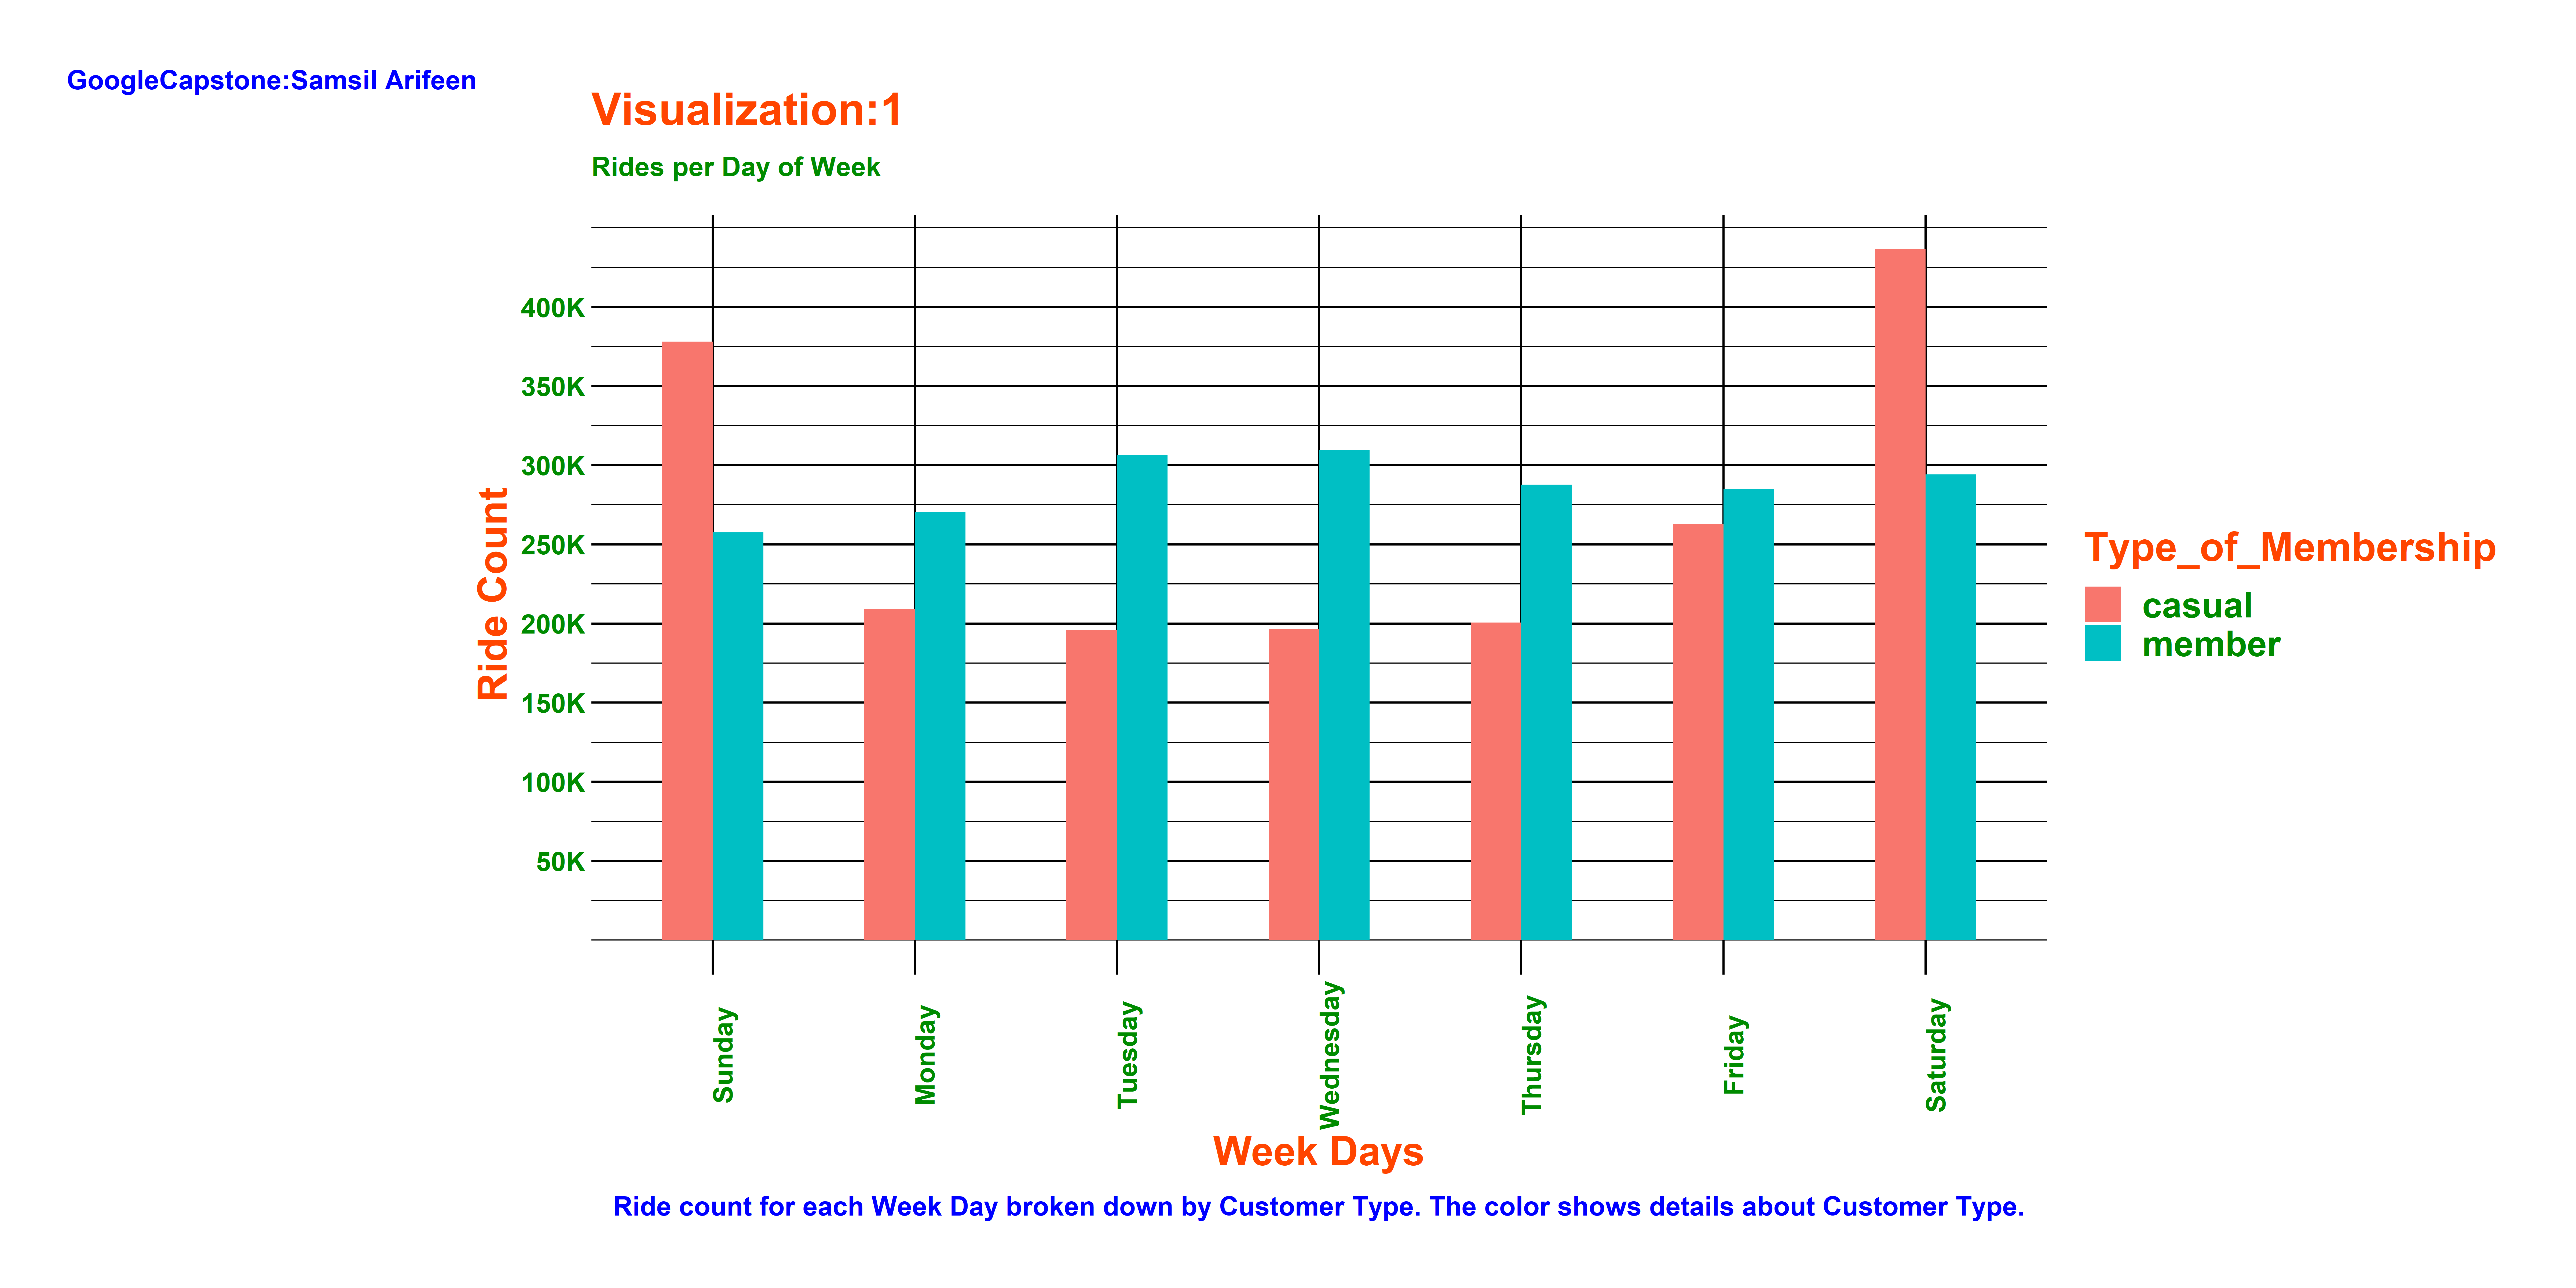
\includegraphics{/home/samsil/Documents/CaseStudy1-Cyclistic/viz1.png}

\hypertarget{visualization2-}{%
\subsubsection{\texorpdfstring{\textbf{Visualization:2-\textgreater{}}}{Visualization:2-\textgreater{}}}\label{visualization2-}}

\textbf{The demand for bike usage in a 24 hour span shows that usage by
annual members peak during rush hour which indicates many members may
use the bikes for commute to and from work especially with the steep
drop after the peak at 6pm. Casual riders are not as volatile as there
is a steady increase throughout the day with a steady decrease after the
peak at 6pm. This plot also supports the previous one and here we can
assume that annual members prefer bikes for there workplace
transportation mostly.}

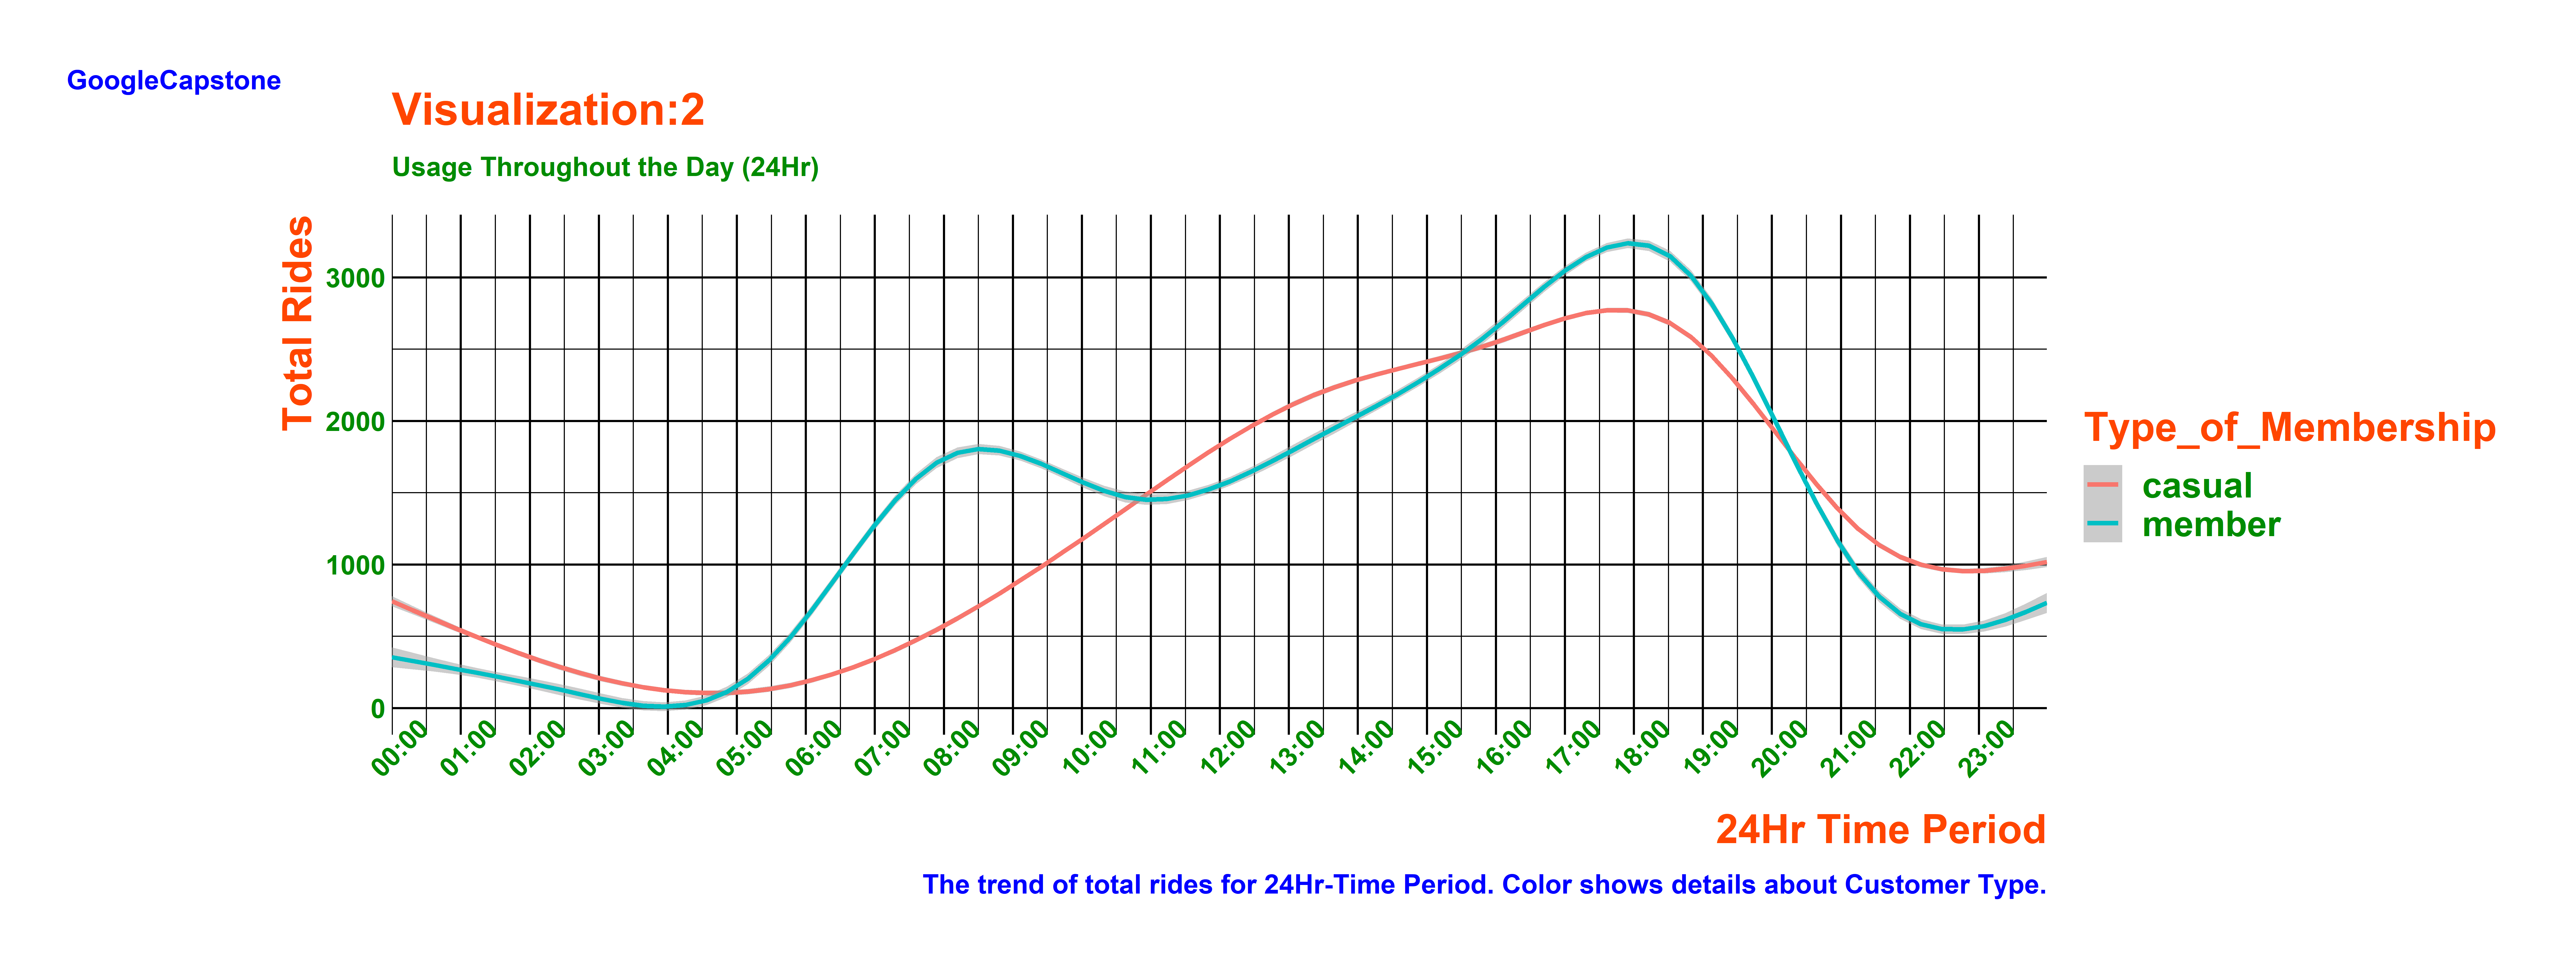
\includegraphics{/home/samsil/Documents/CaseStudy1-Cyclistic/viz2.png}

\hypertarget{visualization3-}{%
\subsubsection{\texorpdfstring{\textbf{Visualization:3-\textgreater{}}}{Visualization:3-\textgreater{}}}\label{visualization3-}}

\textbf{Now, lets see what is the usage status in terms of monthly basis
for bike usage. The summer months bring more riders in both types where
casual usage is a bit higher. On the other hand, casual rider usage is
nearly nonexistent in the winter months than the annual members. There
may be multiple factors which can contribute to this result but annual
members still use the service at a good rate in those months as well. So
we can assume that annual members use bikes in a more steady through out
the year.}

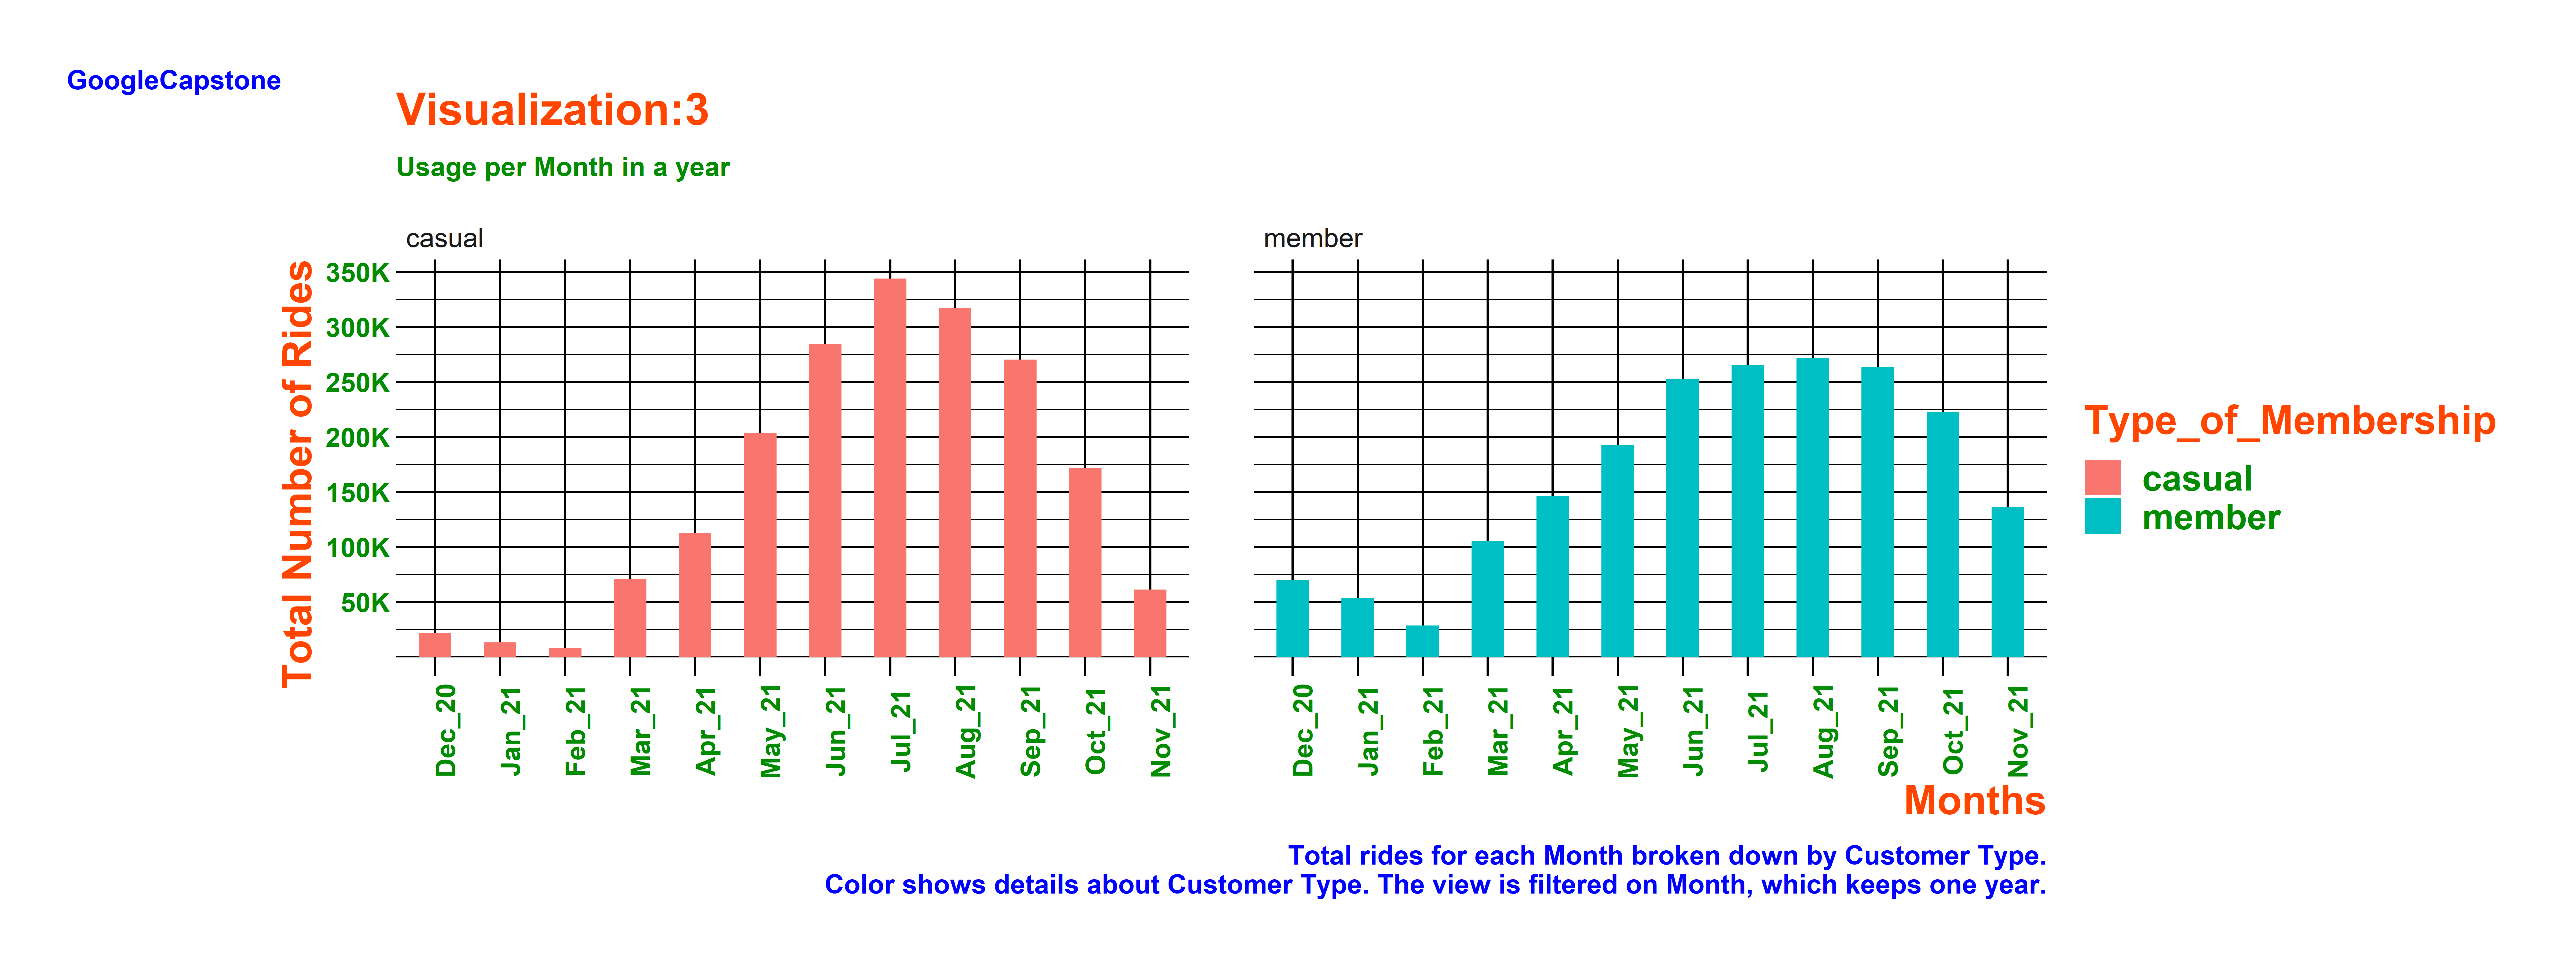
\includegraphics{/home/samsil/Documents/CaseStudy1-Cyclistic/viz3.png}

\hypertarget{visualization4-}{%
\subsubsection{\texorpdfstring{\textbf{Visualization:4-\textgreater{}}}{Visualization:4-\textgreater{}}}\label{visualization4-}}

\textbf{On my fourth plot, i tried to observe the average number of
rides in a week. The average ride length of casual riders is
considerably longer than those of members and with a peak on Saturday
and Sunday. Annual members ride length is near constant length
regardless of day of week. So we can assume that annual members use
bikes in a more steady way through out the week as well.}

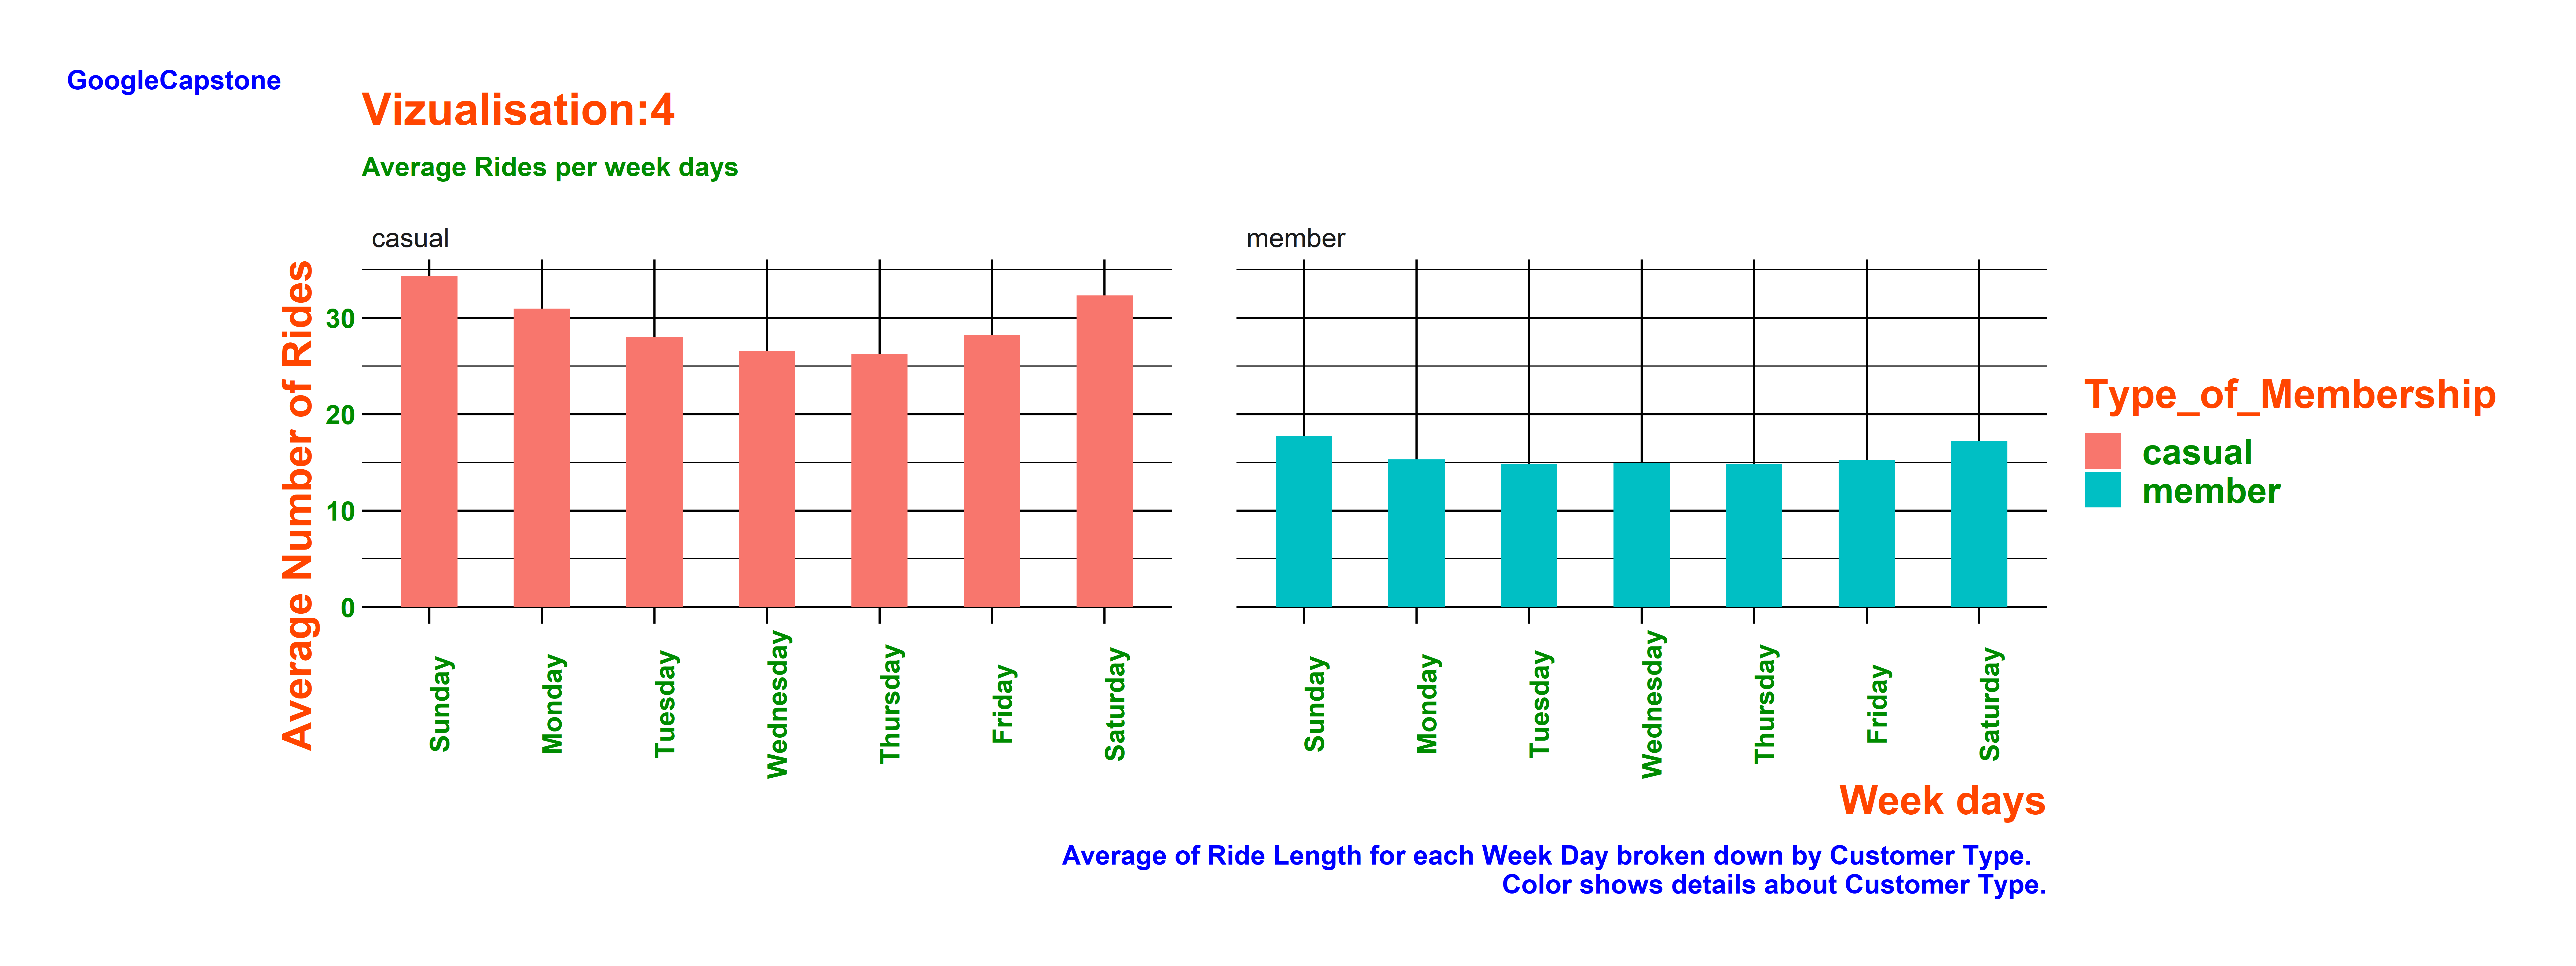
\includegraphics{/home/samsil/Documents/CaseStudy1-Cyclistic/viz4.png}

\hypertarget{visualization5-}{%
\subsubsection{\texorpdfstring{\textbf{Visualization:5-\textgreater{}}}{Visualization:5-\textgreater{}}}\label{visualization5-}}

\textbf{The average ride length by casual riders are still considerably
longer than members even when broken by month also. Casual usage got
higher average usage rate within the middle months as well. On the other
hand, members users' average usage remains lower than casuals but with
steady usage through out the year as well.}

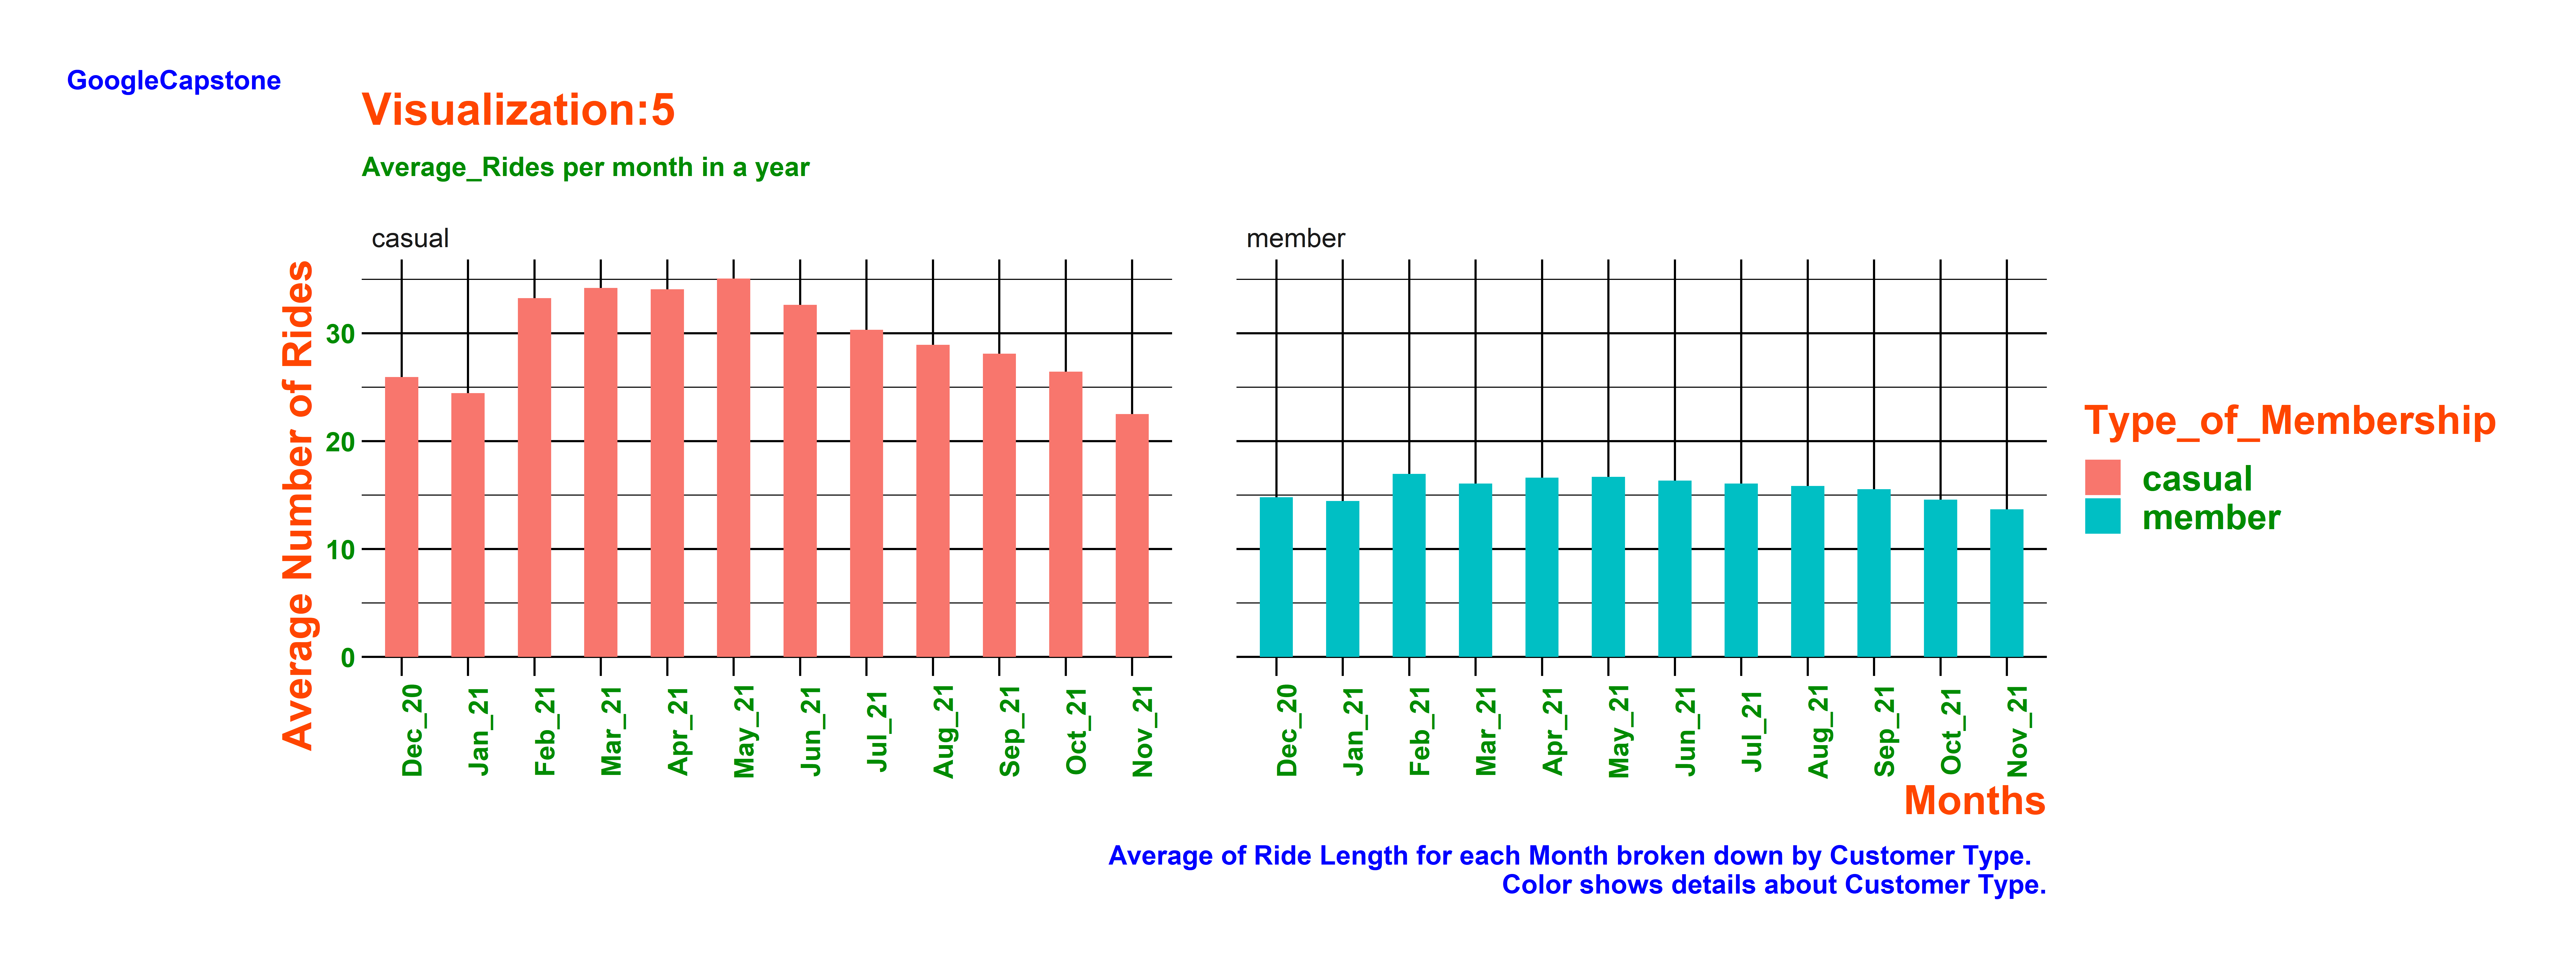
\includegraphics{/home/samsil/Documents/CaseStudy1-Cyclistic/viz5.png}

\hypertarget{visualization6-}{%
\subsubsection{\texorpdfstring{\textbf{Visualization:6-\textgreater{}}}{Visualization:6-\textgreater{}}}\label{visualization6-}}

\textbf{The bike type breakdown shows members use classic bikes more
than casual members.The electric bike usage is nearly identical but
casual riders are more willing to use docked bikes than the member
users. Here it wasn't clear about the definition of `Docked Bike' while
studying the data sets, but it is evident that it is not a preferable or
popular bike service for annual members at all. Both group prefer
classic bikes on top of the other two types.}

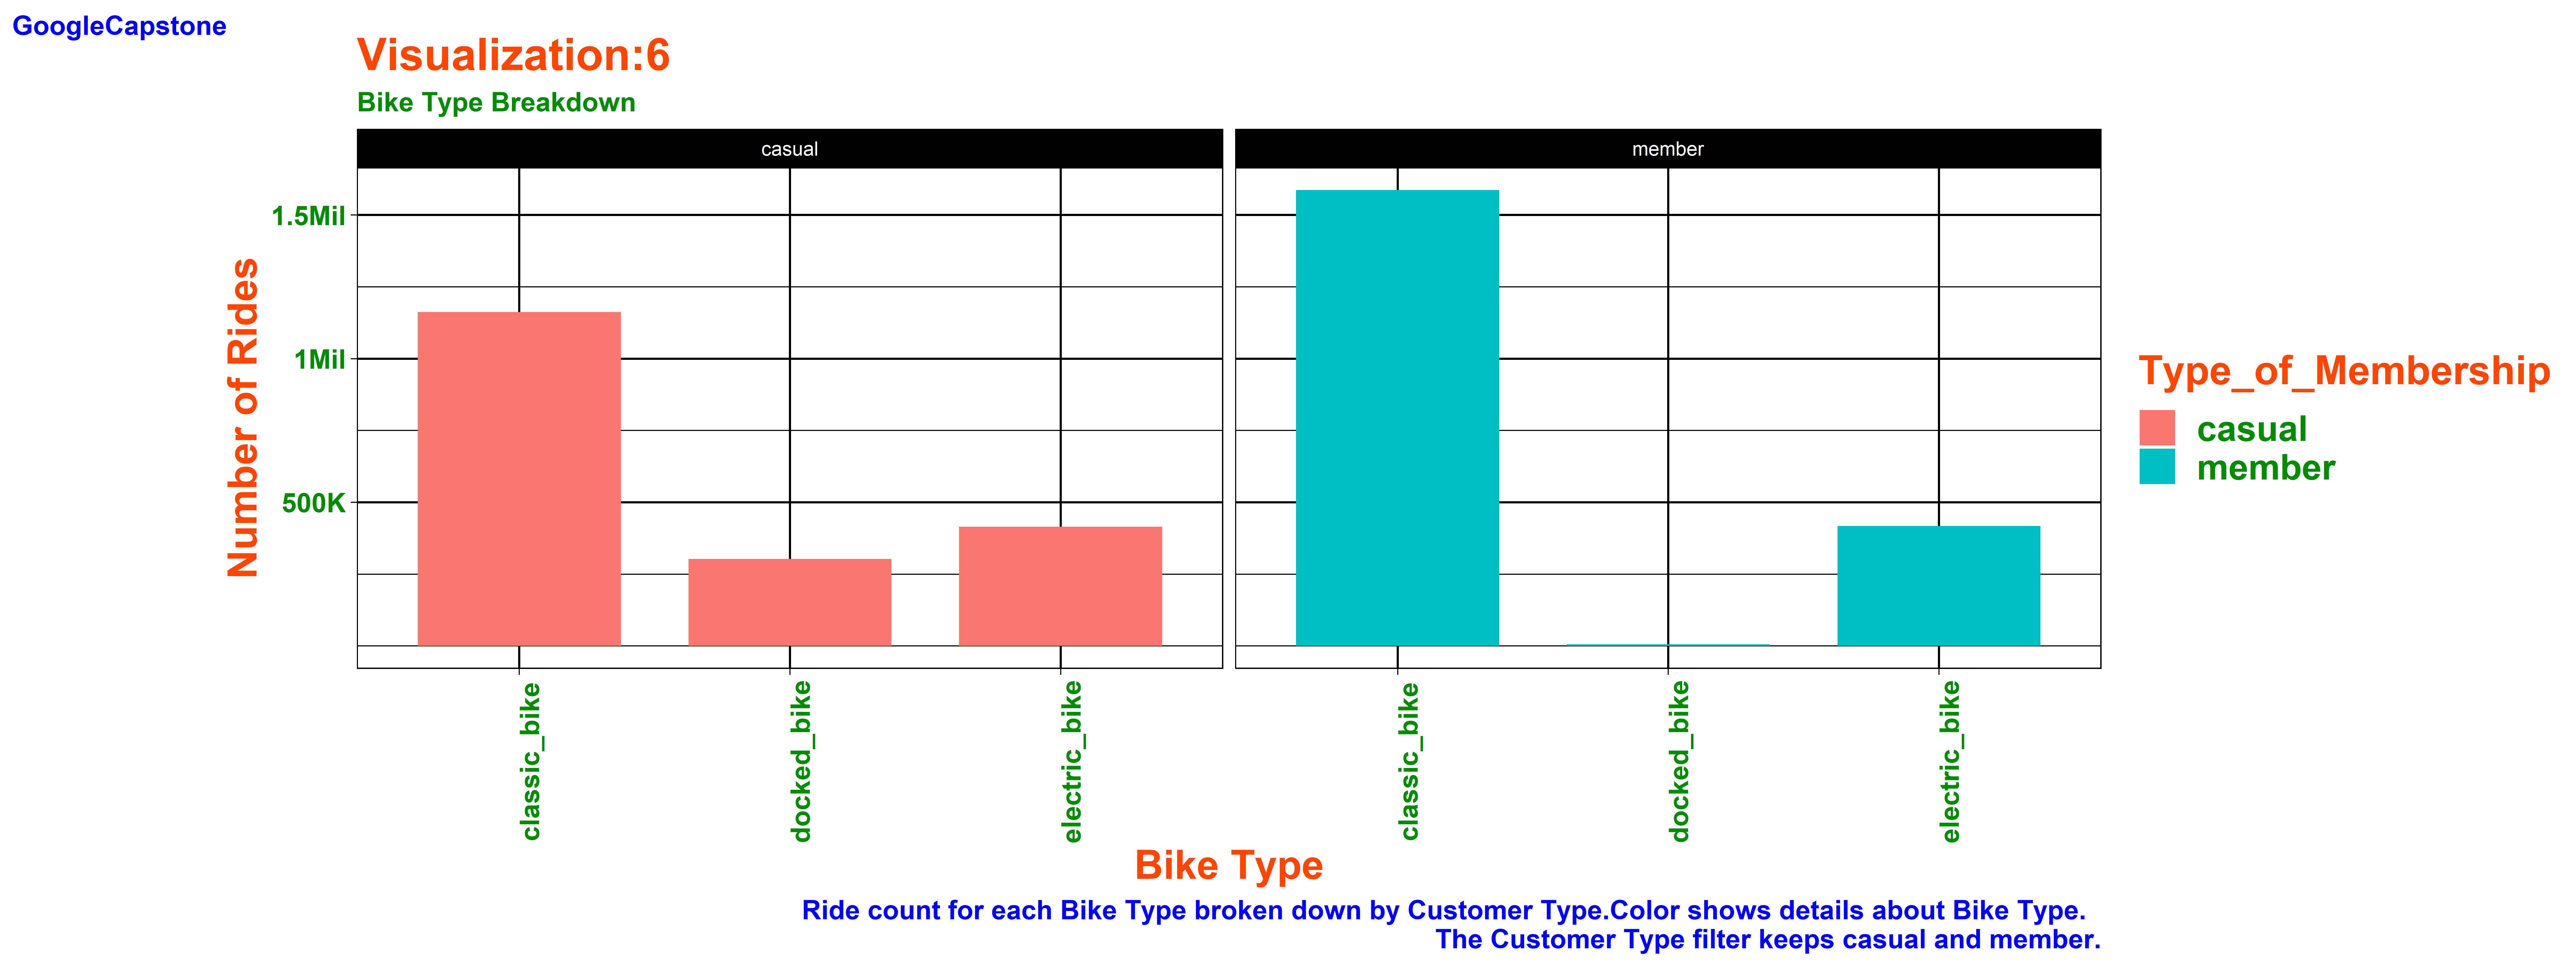
\includegraphics{/home/samsil/Documents/CaseStudy1-Cyclistic/viz6.png}

\hypertarget{visualization7-}{%
\subsubsection{\texorpdfstring{\textbf{Visualization:7-\textgreater{}}}{Visualization:7-\textgreater{}}}\label{visualization7-}}

\textbf{This plot shows us clearly that the total amount of time ridden
by casual riders are greater than that of member riders. Although we
have seen in our previous plots that members usage is more steady both
weekly and yearly basis, but casuals use the bike for more duration than
members.}

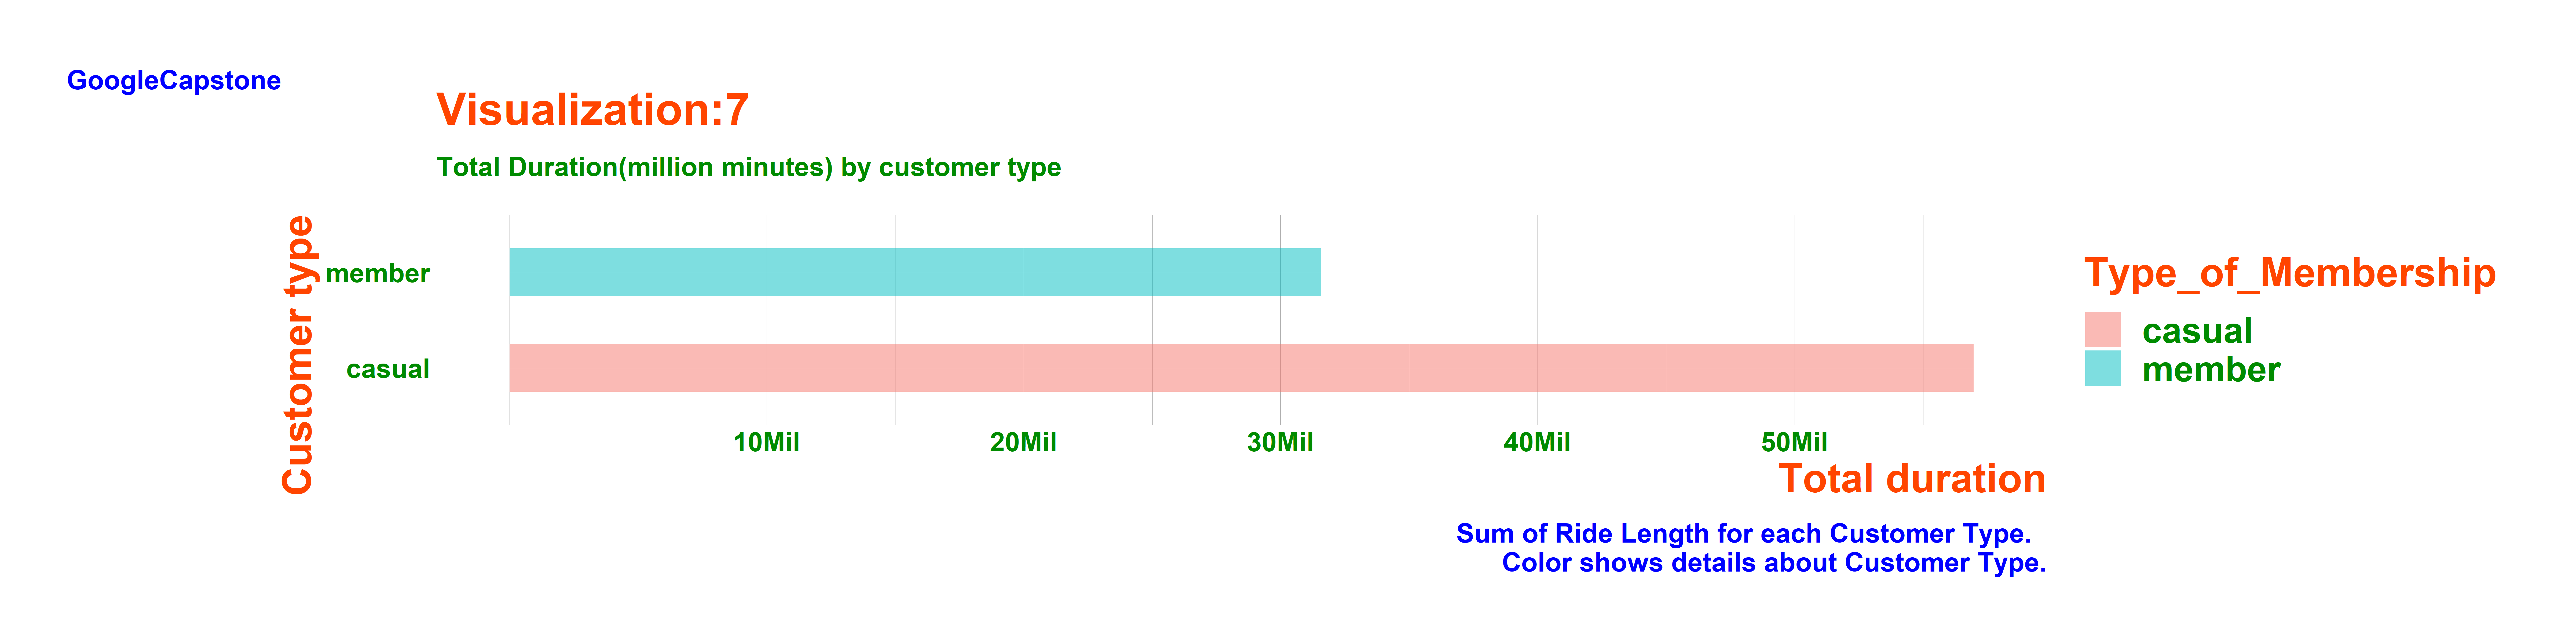
\includegraphics{/home/samsil/Documents/CaseStudy1-Cyclistic/viz7.png}

\hypertarget{visualization8-}{%
\subsubsection{\texorpdfstring{\textbf{Visualization:8-\textgreater{}}}{Visualization:8-\textgreater{}}}\label{visualization8-}}

\textbf{This breakdown bar graph shows weekly frequency distribution of
the member and casual customers with bike types. I had organized week
days in order from Sunday to Saturday. However, this plot shows us few
observations about members and casuals as well. Firstly, members usage
are almost similar throughout the week. We can infer that members are
mostly working people. Secondly, casual usage is slow for weekdays but
weekends are very popular especially Saturday. Thirdly, Docked bike is
the most unpopular for both members and casuals as we observed before as
well. Fourthly, docked bike is not at all popular within annual members
throughout the weekly usage session.}

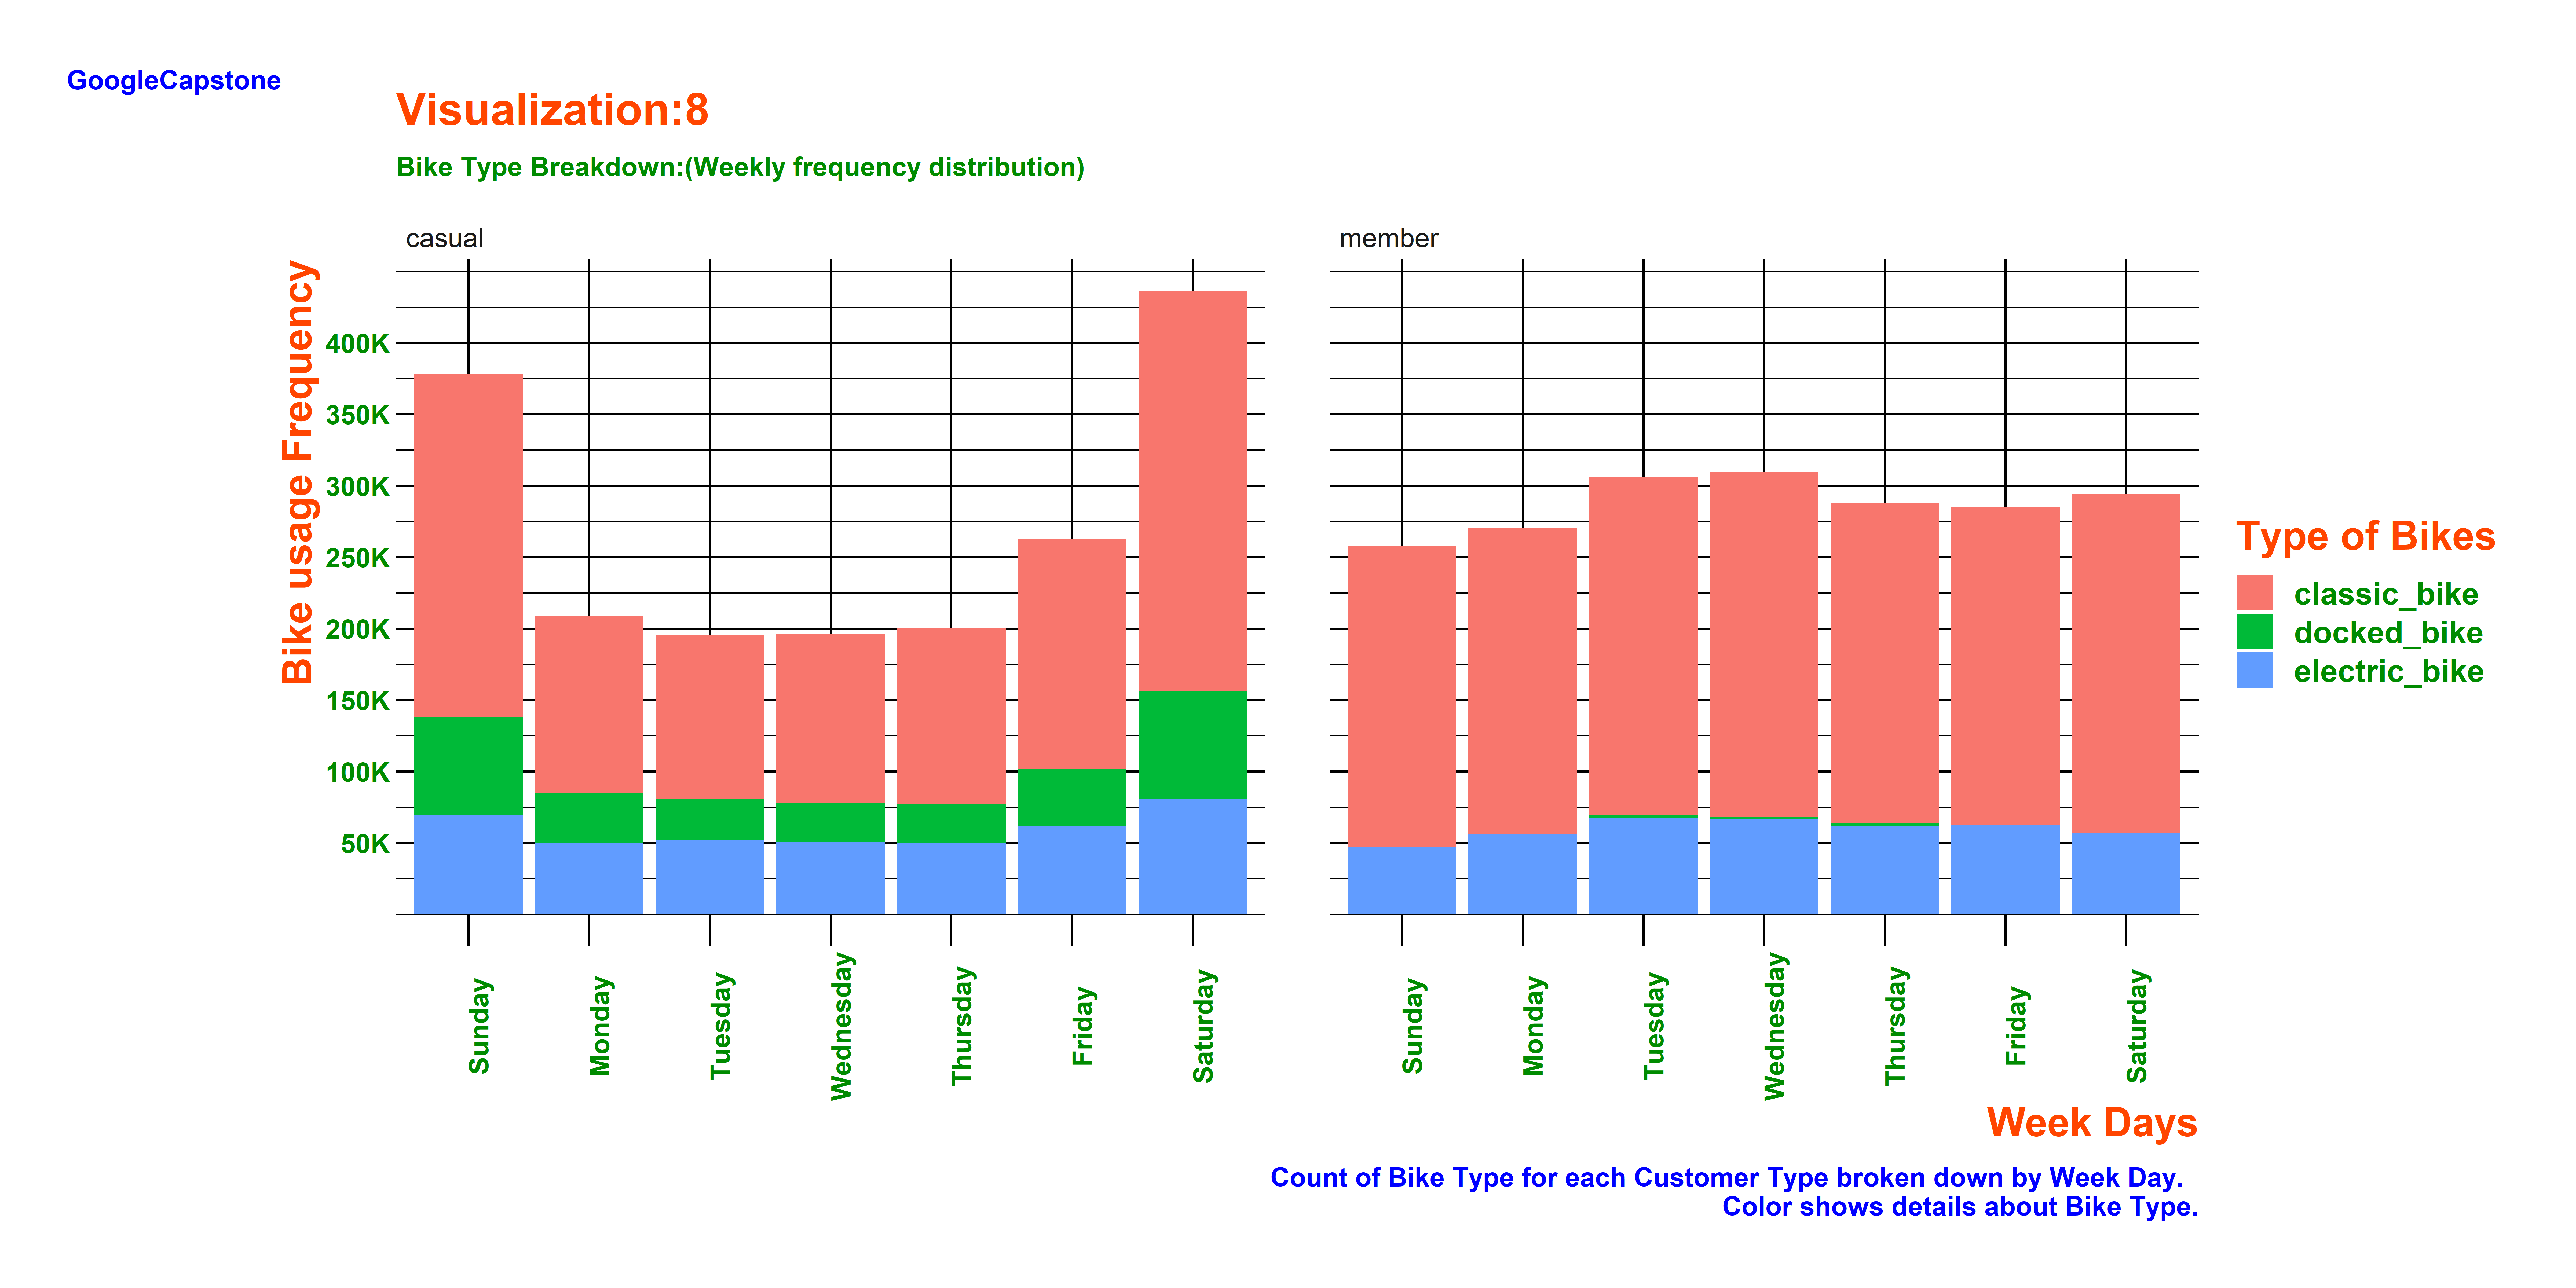
\includegraphics{/home/samsil/Documents/CaseStudy1-Cyclistic/viz8.png}

\hypertarget{visualization9-}{%
\subsubsection{\texorpdfstring{\textbf{Visualization:9-\textgreater{}}}{Visualization:9-\textgreater{}}}\label{visualization9-}}

\textbf{This breakdown bar graph that shows monthly frequency
distribution of the member and casual customers with bike types. I had
organized months in order from December,2020 till November, 2021 as per
my data sets for one year. However, this plot shows us a few
observations also about members and casuals. Casual usage is higher than
the members specially within the middle months. Both user group mostly
choose classic bike than other two types all over the year. However, it
is evident that member usage is higher even in the winter seasons and
they also maintains a steady usage frequency all over the year than the
casuals. It also supports the assumption that docked bike is not popular
at all within the members through out the year as well.}

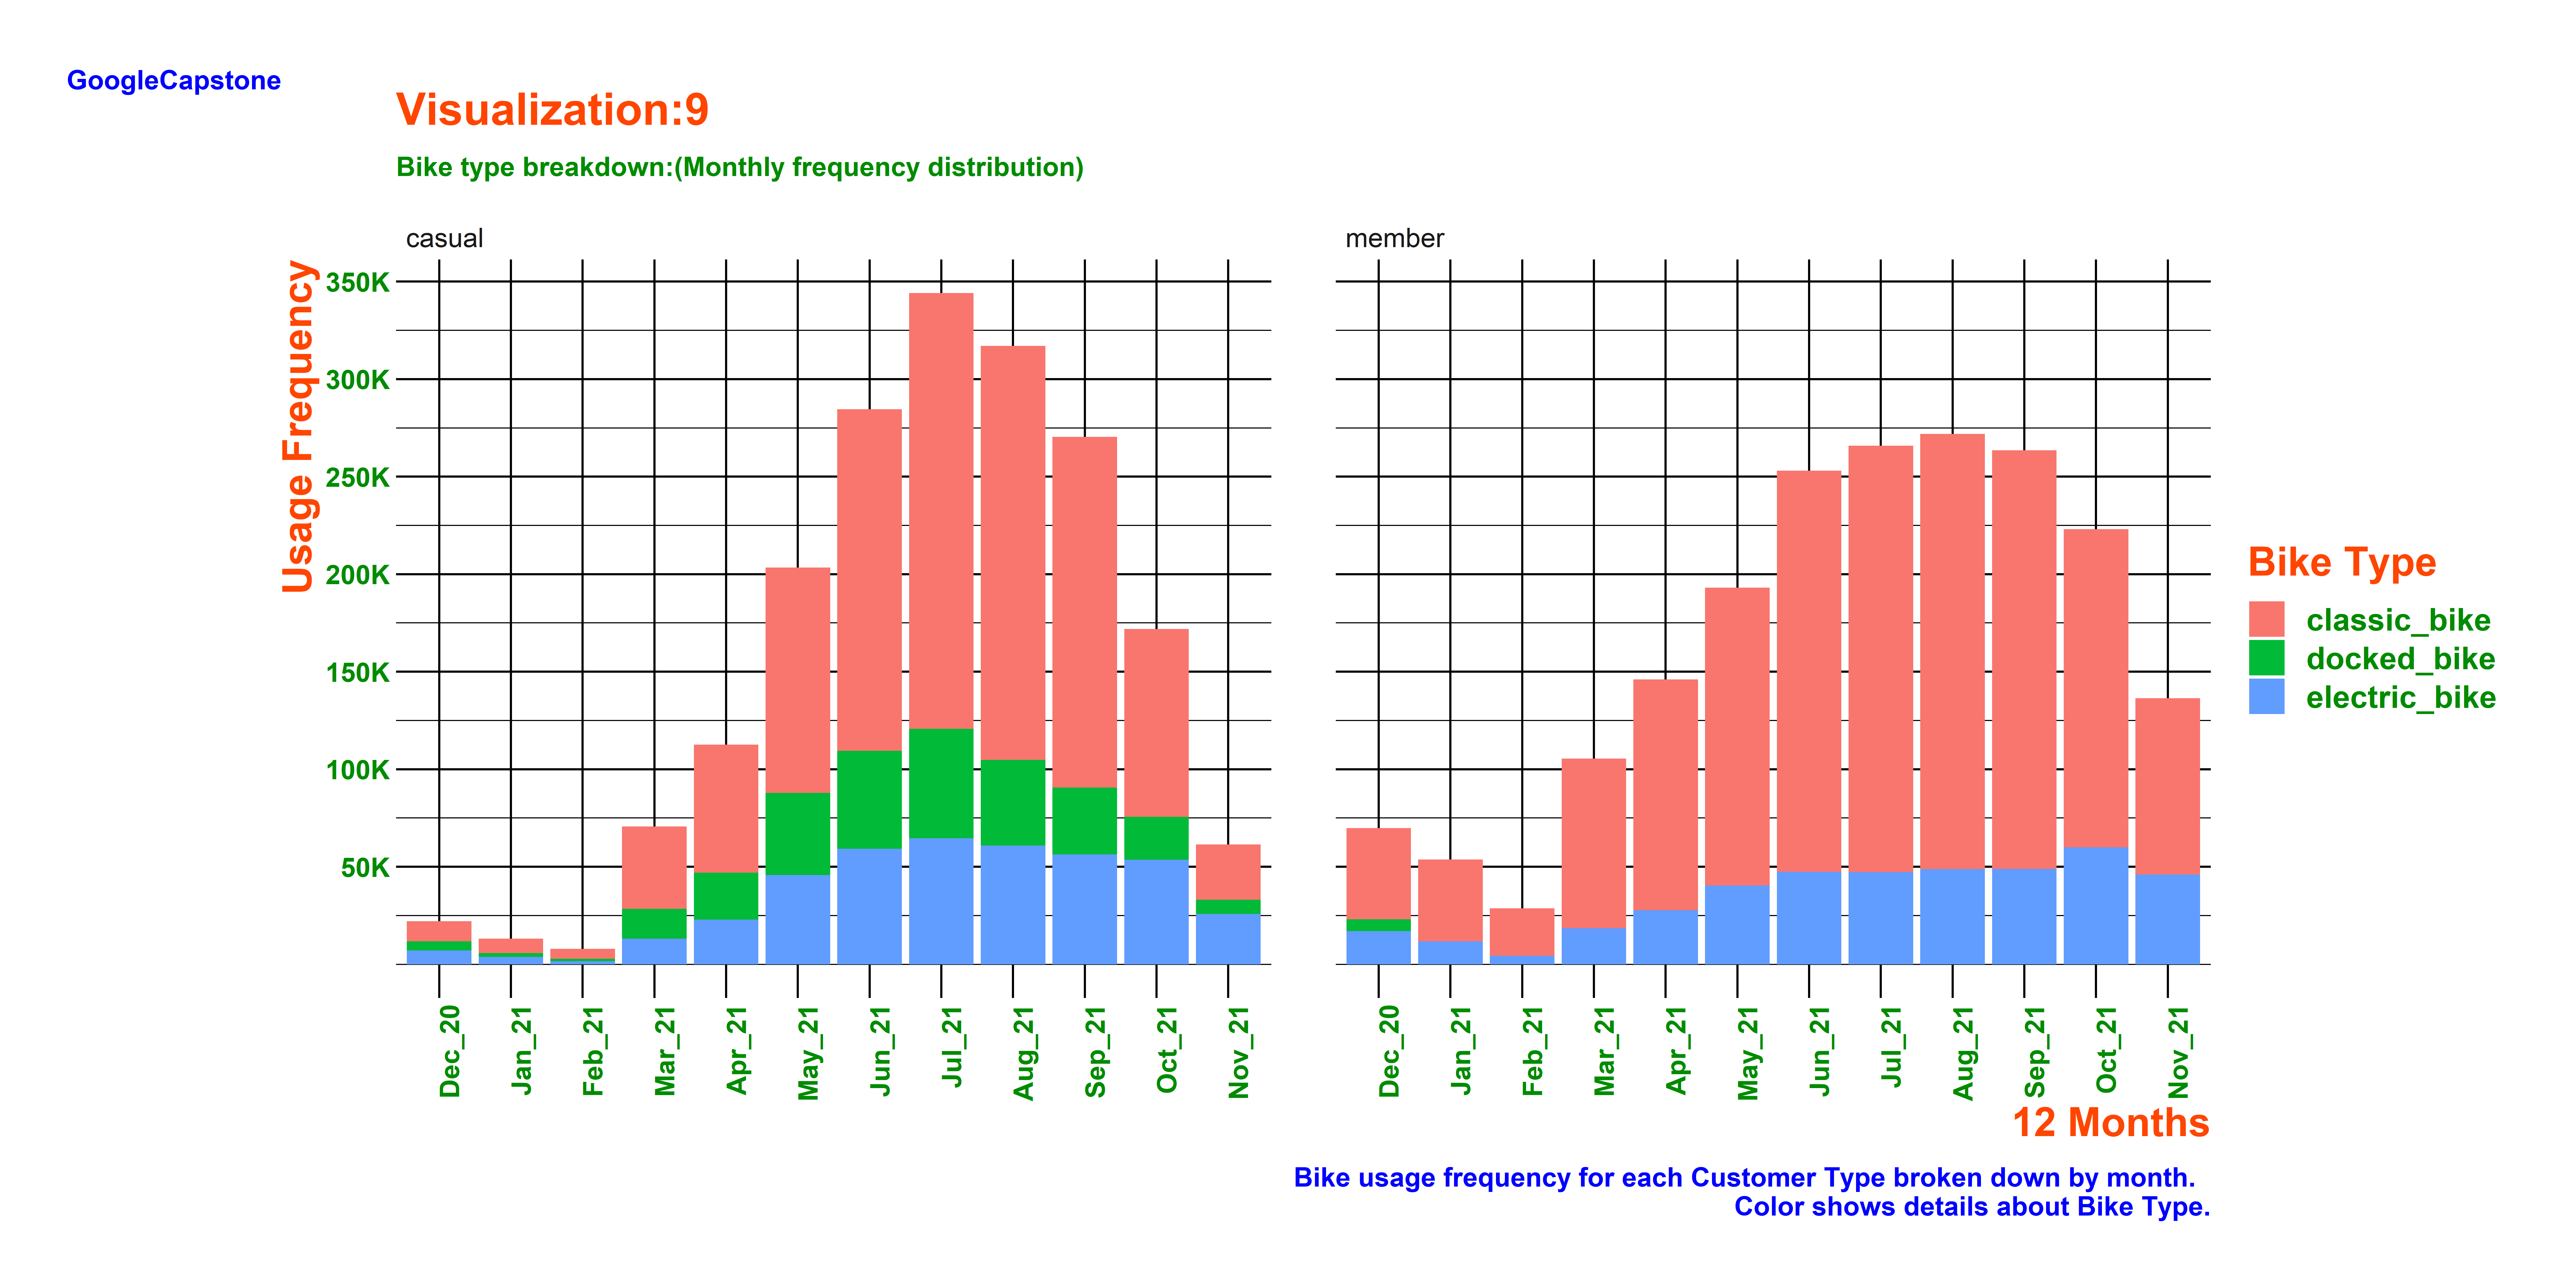
\includegraphics{/home/samsil/Documents/CaseStudy1-Cyclistic/viz9.png}

\hypertarget{visualization10-}{%
\subsubsection{\texorpdfstring{\textbf{Visualization:10-\textgreater{}}}{Visualization:10-\textgreater{}}}\label{visualization10-}}

\textbf{Now let's observe ride duration behavior for member and casuals
by a histogram and we will observe the density in terms of usage
behavior as well. For this I have filtered the duration times to less
than 100 minutes for a better density. Only observation here is that
members tend to take short trips than casuals. Or casual users' trip
duration is longer than members. On the other hand, we can also say that
member users' ride count is higher within shorter duration.}

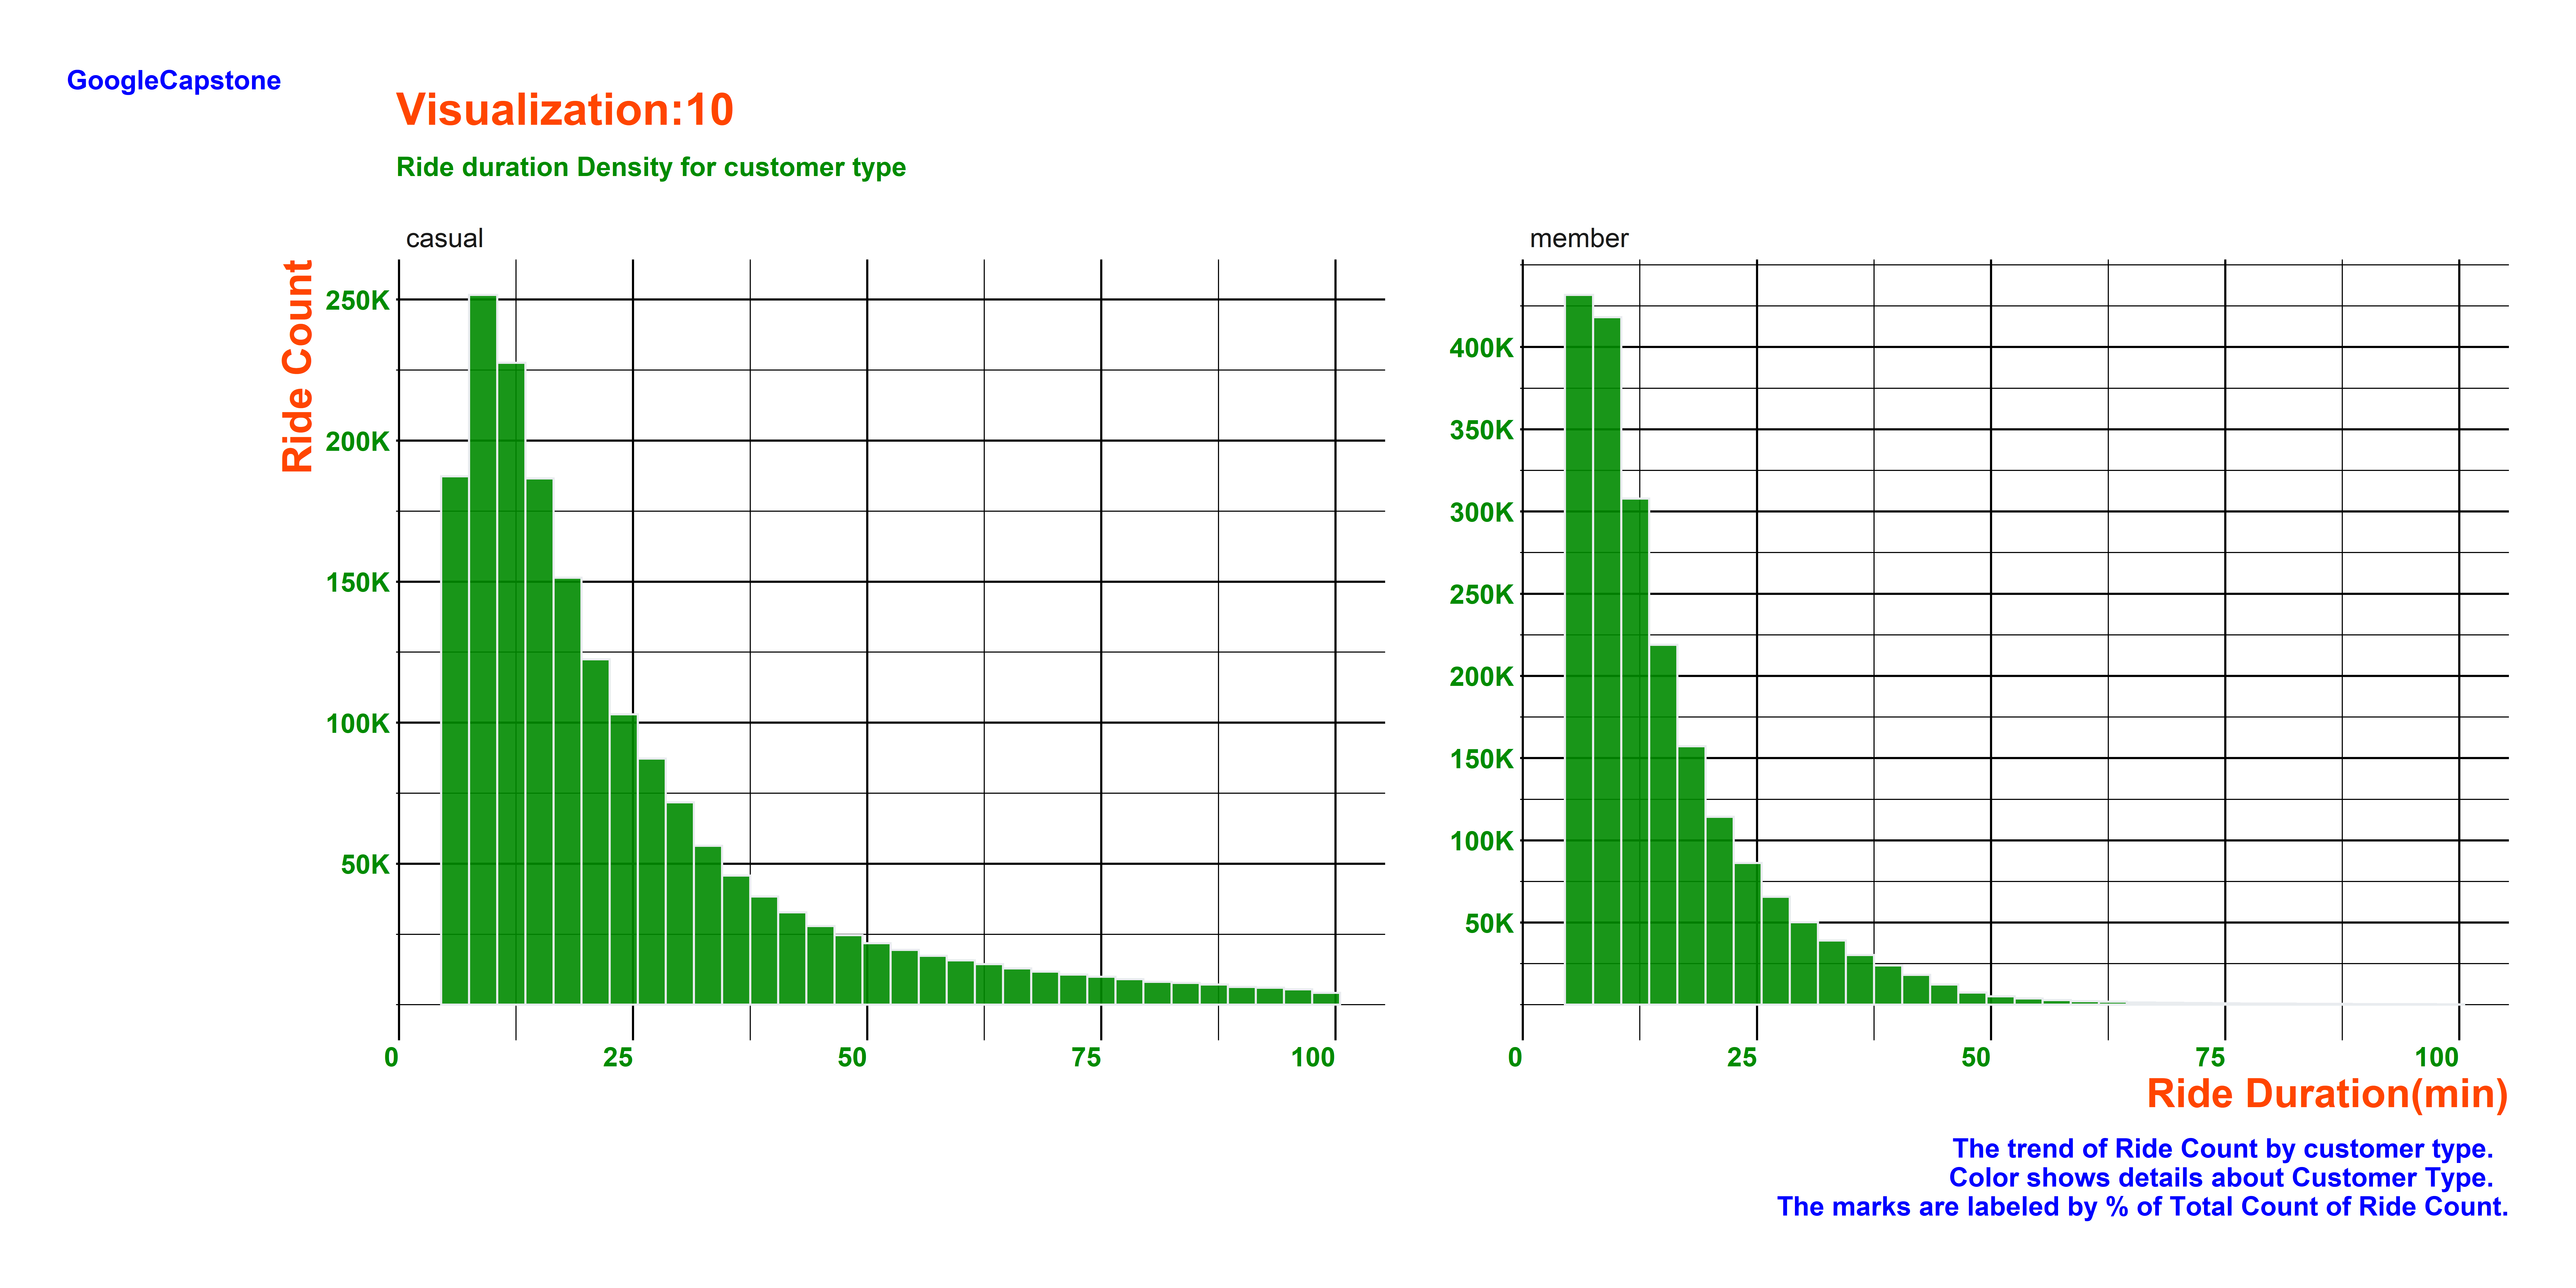
\includegraphics{/home/samsil/Documents/CaseStudy1-Cyclistic/viz10.png}

\hypertarget{visualization11-}{%
\subsubsection{\texorpdfstring{\textbf{Visualization:11-\textgreater{}}}{Visualization:11-\textgreater{}}}\label{visualization11-}}

\textbf{This visualization is a histogram using data from the `time'
column that we have created right after the data cleaning in order to
investigate whether there was a difference within the start time for
trips or rides between casual and member customer type. There was
noticeable higher number of start time for member-users in early morning
hours between 7am till 8am specifically.This also support the
observation that members are using the bikes mostly for commute to work.
On the other hand, there is another high pick noticeable for members
again later in the evening that is 5pm to 7pm to be specific. Which
indicates end of work day. However, for casuals, it seems that their
bike usage is mostly during the later part of the day and afternoon.
Here a noticeably higher number of rides being started by casual users
between 1pm to 2pm followed by the highest pick at 4pm. In that case we
can assume that casual users mostly use the bikes for a leisure.}

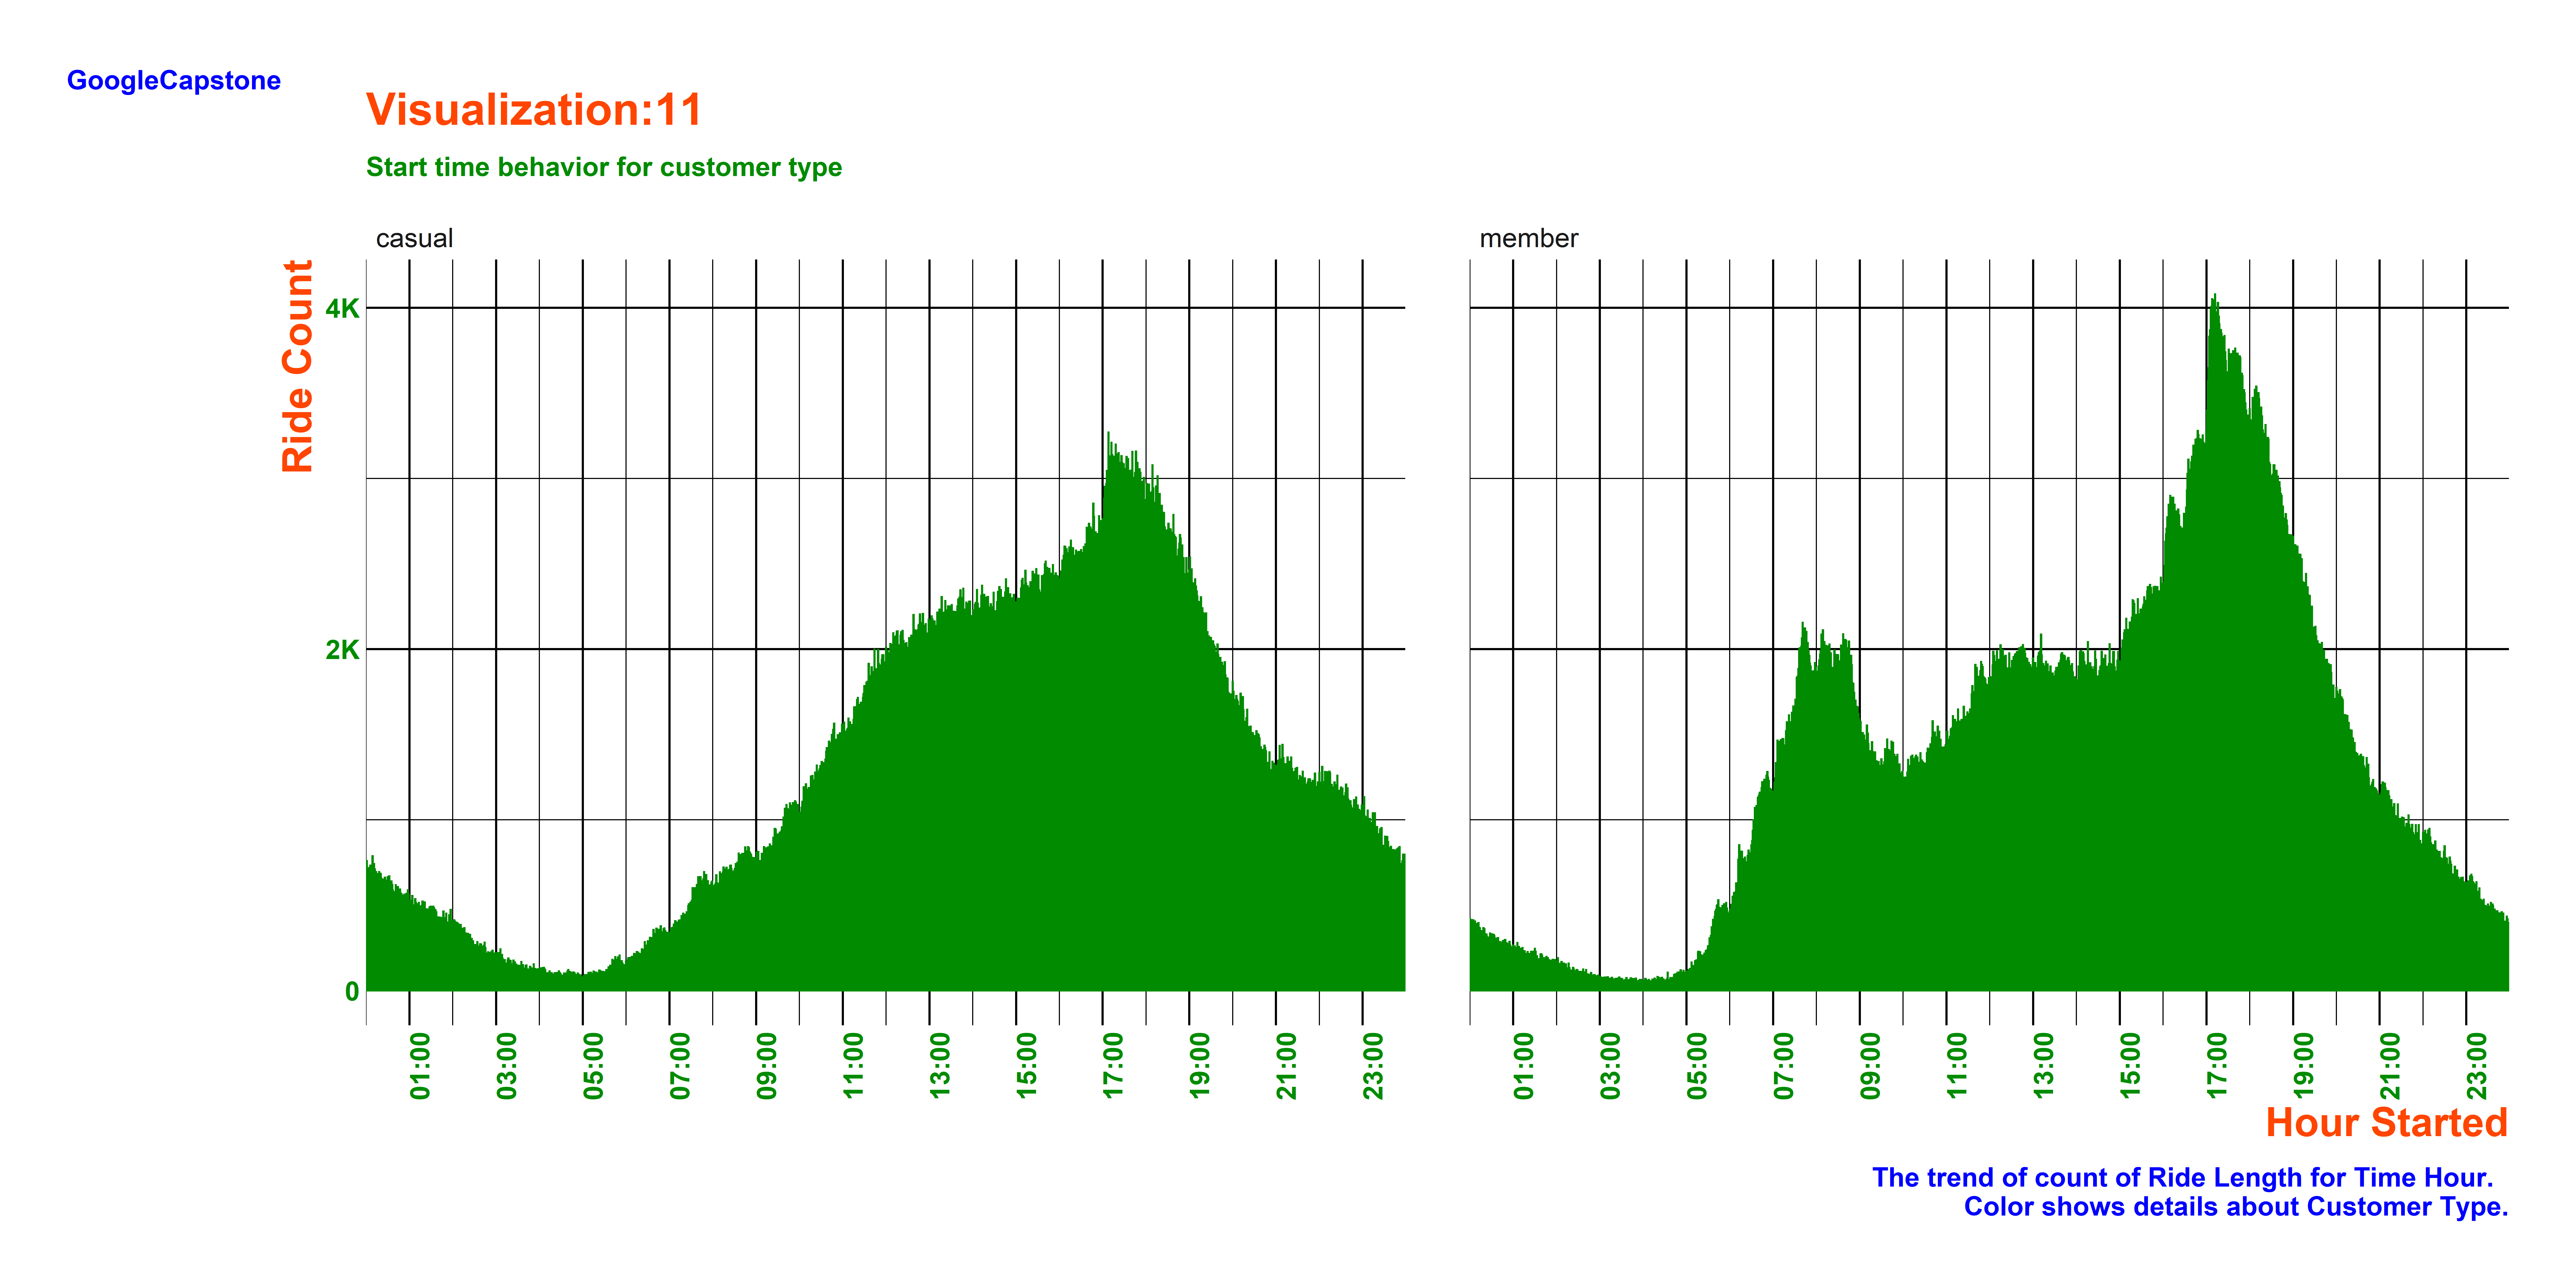
\includegraphics{/home/samsil/Documents/CaseStudy1-Cyclistic/viz11.png}

\hypertarget{phase-6-act}{%
\section{\texorpdfstring{\textbf{Phase 6:
ACT}}{Phase 6: ACT}}\label{phase-6-act}}

\hypertarget{key-takeaways-}{%
\subsubsection{\texorpdfstring{\textbf{Key
Takeaways-\textgreater{}}}{Key Takeaways-\textgreater{}}}\label{key-takeaways-}}

\begin{itemize}
\item
  \textbf{Annual members mainly use the bikes for regular commutes while
  casual users for leisure on weekends or summer months in a year.}
\item
  \textbf{Annual Members bike usage is more steady through out a day of
  weeks or even in months of a year than casual users bike usage.}
\item
  \textbf{Both casual and annual members prefer classic bikes than other
  two types of bikes.}
\item
  \textbf{Annual members mainly use classic bikes and rarely use docked
  bikes but casual riders are more open to riding all kinds of bikes.}
\item
  \textbf{Casual users ride nearly 50\% longer than the annual members
  in terms of ride duration in total.}
\item
  \textbf{Casual riders do not use the service during the winter months
  as much as annual members.}
\end{itemize}

\hypertarget{recommendations-}{%
\subsubsection{\texorpdfstring{\textbf{Recommendations-\textgreater{}}}{Recommendations-\textgreater{}}}\label{recommendations-}}

\begin{itemize}
\item
  \textbf{To reach the most riders, marketing should be targeted for the
  busiest casual rider days (Friday, Saturday and Sunday), busiest hours
  (afternoon) and the most popular months (June, July and August).}
\item
  \textbf{Run promotions for annual memberships during the winter months
  to boost sales and try to convert casual riders into annual members.}
\item
  \textbf{Decrease the price of single-fare and full-day passes from
  Monday through Friday to boost casual ridership during the work hour.}
\item
  \textbf{Single-fare and full-day passes' sale can be increased on
  Saturday and Sunday to entice customers to convert from casual
  ridership into annual membership.}
\end{itemize}

\hypertarget{additional-analysis-for-future}{%
\subsubsection{\texorpdfstring{\textbf{Additional analysis for
future}}{Additional analysis for future}}\label{additional-analysis-for-future}}

\begin{itemize}
\item
  \textbf{Age and gender - This data is missing as these could show the
  demographics of the existing customers which could be used to target
  others in similar groups.}
\item
  \textbf{Marital status - This data could be used for promotional use
  to target entire families and not just individuals as well.}
\item
  \textbf{Pricing of plans - This missing data can be used to optimize
  the cost benefit analysis for existing customers and potential new
  ones.}
\item
  \textbf{Income range - This data could be used for targeting potential
  customers in certain income ranges and/or neighborhoods.}
\end{itemize}

\textbf{------------------------------------------------------------------------------------------------------End
of Case
Study----------------------------------------------------------------}

\end{document}
